%%
%% This is file `sample-acmsmall.tex',
%% generated with the docstrip utility.
%%
%% The original source files were:
%%
%% samples.dtx  (with options: `all,journal,bibtex,acmsmall')
%% 
%% IMPORTANT NOTICE:
%% 
%% For the copyright see the source file.
%% 
%% Any modified versions of this file must be renamed
%% with new filenames distinct from sample-acmsmall.tex.
%% 
%% For distribution of the original source see the terms
%% for copying and modification in the file samples.dtx.
%% 
%% This generated file may be distributed as long as the
%% original source files, as listed above, are part of the
%% same distribution. (The sources need not necessarily be
%% in the same archive or directory.)
%%
%%
%% Commands for TeXCount
%TC:macro \cite [option:text,text]
%TC:macro \citep [option:text,text]
%TC:macro \citet [option:text,text]
%TC:envir table 0 1
%TC:envir table* 0 1
%TC:envir tabular [ignore] word
%TC:envir displaymath 0 word
%TC:envir math 0 word
%TC:envir comment 0 0
%%
%% The first command in your LaTeX source must be the \documentclass
%% command.
%%
%% For submission and review of your manuscript please change the
%% command to \documentclass[manuscript, screen, review]{acmart}.
%%
%% When submitting camera ready or to TAPS, please change the command
%% to \documentclass[sigconf]{acmart} or whichever template is required
%% for your publication.
%%
%%
\documentclass[acmsmall]{acmart}
%%
%% \BibTeX command to typeset BibTeX logo in the docs
\AtBeginDocument{%
  \providecommand\BibTeX{{%
    Bib\TeX}}}



%% Rights management information.  This information is sent to you
%% when you complete the rights form.  These commands have SAMPLE
%% values in them; it is your responsibility as an author to replace
%% the commands and values with those provided to you when you
%% complete the rights form.
\setcopyright{rightsretained}
%\copyrightyear{2026}
\acmYear{2026}
%\acmDOI{XXXXXXX.XXXXXXX}

%%
%% These commands are for a JOURNAL article.
\acmJournal{JACM}
\acmVolume{1}
\acmNumber{1}
\acmArticle{1}

%%packages
%\usepackage{url}
%\usepackage[edges]{forest}
%\forestset{
%  default preamble = {forked edges},   % runs after a root node exists
%}
%\usetikzlibrary{trees,shapes.symbols}
%\usepackage{graphicx} % for resizebox
%\usepackage{xcolor}
%\definecolor{hidden-draw}{gray}{0.7}
%\useforestlibrary{edges}


\usepackage{url}
\usepackage{forest}
\usepackage{hyperref}
\forestset{forked edges}
\usetikzlibrary{trees}
\usepackage{graphicx} % for resizebox
\usepackage{xcolor}
\usepackage[table]{xcolor}
\definecolor{recnode}{HTML}{F7D1BA}      
\definecolor{llmbranch}{HTML}{fa8998}    
\definecolor{seqbranch}{HTML}{b1d7fa}
\definecolor{multibranch}{HTML}{aedda4}  
\definecolor{persbranch}{HTML}{fece6d}  
\definecolor{explbranch}{HTML}{dcb2ff}  
\definecolor{privbranch}{HTML}{91dedc} 
\definecolor{effbranch}{HTML}{ffb3c6} 

% === Forest style definitions ===
\forestset{
  forked edges/.style={
    for tree={
      edge path={
        \noexpand\path [draw, \forestoption{edge}]
        (!u.parent anchor) -- +(5pt,0) |- (.child anchor)\forestoption{edge label};
      },
      parent anchor=east,
      child anchor=west,
    }
  },
  folder/.style={
    draw,
    rounded corners,
    fill=gray!10
  },
  hidden-draw/.style={draw},
  root style/.style={fill=gray!20},
  entiteschild style/.style={fill=blue!10},
  entitesgrandchild style/.style={fill=blue!5},
  entitiesgreatgrandchild style/.style={fill=white},
  entitesleaf style/.style={},
  relationschild style/.style={fill=green!10},
  relationsgrandchild style/.style={fill=green!5},
  relationsgreatgrandchild style/.style={fill=white},
  relationsleaf style/.style={},
  sememeschild style/.style={fill=orange!10},
  sememesgrandchild style/.style={fill=orange!5},
  sememesgreatgrandchild style/.style={fill=white},
  sememesleaf style/.style={},
  eventschild style/.style={fill=purple!10},
  eventsgrandchild style/.style={fill=purple!5},
  eventsgreatgrandchild style/.style={fill=white},
  eventsleaf style/.style={},
  conceptschild style/.style={fill=red!10},
  conceptsgrandchild style/.style={fill=red!5},
  conceptsgreatgrandchild style/.style={fill=white},
  conceptsleaf style/.style={},
}

\usepackage{enumitem}

\newlist{paralist}{enumerate}{1}
\setlist[paralist,1]{label=\arabic*., leftmargin=*, itemsep=1em}

%%
%% Submission ID.
%% Use this when submitting an article to a sponsored event. You'll
%% receive a unique submission ID from the organizers
%% of the event, and this ID should be used as the parameter to this command.
%%\acmSubmissionID{123-A56-BU3}

%%
%% For managing citations, it is recommended to use bibliography
%% files in BibTeX format.
%%
%% You can then either use BibTeX with the ACM-Reference-Format style,
%% or BibLaTeX with the acmnumeric or acmauthoryear sytles, that include
%% support for advanced citation of software artefact from the
%% biblatex-software package, also separately available on CTAN.
%%
%% Look at the sample-*-biblatex.tex files for templates showcasing
%% the biblatex styles.
%%

%%
%% The majority of ACM publications use numbered citations and
%% references.  The command \citestyle{authoryear} switches to the
%% "author year" style.
%%
%% If you are preparing content for an event
%% sponsored by ACM SIGGRAPH, you must use the "author year" style of
%% citations and references.
%% Uncommenting
%% the next command will enable that style.
%%\citestyle{acmauthoryear}

\usepackage{booktabs}
\usepackage{multirow}
\usepackage{threeparttable}
\usepackage{pifont}
\newcommand{\cmark}{\ding{51}}
\newcommand{\xmark}{\ding{55}}

%%packages
\usepackage{url}

%%
%% end of the preamble, start of the body of the document source.
\begin{document}

%%
%% The "title" command has an optional parameter,
%% allowing the author to define a "short title" to be used in page headers.
\title{Quantifying the Gaps: A Systematic Taxonomy of Bias and Imbalance in 96 Multilingual AI Benchmarks \& Datasets}

%%
%% The "author" command and its associated commands are used to define
%% the authors and their affiliations.
%% Of note is the shared affiliation of the first two authors, and the
%% "authornote" and "authornotemark" commands
%% used to denote shared contribution to the research.
% \author{Ben Trovato}
% \authornote{Both authors contributed equally to this research.}
% \email{trovato@corporation.com}
% \orcid{1234-5678-9012}
% \author{G.K.M. Tobin}
% \authornotemark[1]
% \email{webmaster@marysville-ohio.com}
% \affiliation{%
%   \institution{Institute for Clarity in Documentation}
%   \city{Dublin}
%   \state{Ohio}
%   \country{USA}
% }


% \author{Valerie B\'eranger}
% \affiliation{%
%   \institution{Inria Paris-Rocquencourt}
%   \city{Rocquencourt}
%   \country{France}
% }

\author{Sankalp Jajee}
\email{jajee@musc.edu}
\affiliation{%
\institution{Medical University of South Carolina}
\city{Charleston}
\state{South Carolina}
\country{USA}}

\author{Tanisha Shaw}
\affiliation{%
  \institution{LASALLE College of the Arts}
  \city{Singapore}
  \country{Singapore}}
\email{tanishashaw1512@gmail.com}

\author{Vatsalya Soni}
\affiliation{%
  \institution{Delhi Technological University}
  \city{Delhi}
  \country{India}}
\email{vatsalyasoni20@gmail.com}






%%
%% By default, the full list of authors will be used in the page
%% headers. Often, this list is too long, and will overlap
%% other information printed in the page headers. This command allows
%% the author to define a more concise list
%% of authors' names for this purpose.
\renewcommand{\shortauthors}{Jajee et al.}

%%
%% The abstract is a short summary of the work to be presented in the
%% article.
\begin{abstract}

The rapid growth of multilingual AI has created a fragmented and poorly understood evaluation landscape, leading to distorted signals of progress and hindering the development of truly global models. This paper introduces the first systematic, capability-aligned taxonomy of multilingual evaluation to address this critical infrastructure gap. We unify and deconstruct 96 resources from 2018–2025—including 65 benchmarks and 31 datasets—along five critical dimensions: data origin, linguistic resource tier, task class, cultural specificity, and inference paradigm. Our taxonomy provides a powerful diagnostic tool, moving beyond qualitative assumptions to quantify the field's structural flaws for the first time. The analysis reveals profound resource imbalances, with low-resource languages constituting a mere 6.2\% of evaluation benchmarks. It also uncovers a pervasive lack of cultural grounding (55.4\% of benchmarks are culturally non-specific) and a heavy reliance on translated data (26.2\% of benchmarks), which introduces performance-distorting artifacts. By organizing the field, our framework also surfaces surprising performance dynamics, such as the consistent outperformance of the "Translate-Test" paradigm in certain low-resource settings. By reframing evaluation as foundational infrastructure rather than a disconnected aggregation of datasets, this work establishes a principled, evidence-based roadmap. It provides the clarity needed to move beyond superficial leaderboards and begin building the next generation of AI that is not just multilingual in theory, but globally reliable and culturally inclusive in practice.



\end{abstract}

%%
%% The code below is generated by the tool at http://dl.acm.org/ccs.cfm.
%% Please copy and paste the code instead of the example below.
%%
% \begin{CCSXML}
% <ccs2012>
%  <concept>
%   <concept_id>00000000.0000000.0000000</concept_id>
%   <concept_desc>Do Not Use This Code, Generate the Correct Terms for Your Paper</concept_desc>
%   <concept_significance>500</concept_significance>
%  </concept>
%  <concept>
%   <concept_id>00000000.00000000.00000000</concept_id>
%   <concept_desc>Do Not Use This Code, Generate the Correct Terms for Your Paper</concept_desc>
%   <concept_significance>300</concept_significance>
%  </concept>
%  <concept>
%   <concept_id>00000000.00000000.00000000</concept_id>
%   <concept_desc>Do Not Use This Code, Generate the Correct Terms for Your Paper</concept_desc>
%   <concept_significance>100</concept_significance>
%  </concept>
%  <concept>
%   <concept_id>00000000.00000000.00000000</concept_id>
%   <concept_desc>Do Not Use This Code, Generate the Correct Terms for Your Paper</concept_desc>
%   <concept_significance>100</concept_significance>
%  </concept>
% </ccs2012>
% \end{CCSXML}

\begin{CCSXML}
<ccs2012>
<concept>
<concept_id>10010147.10010257</concept_id>
<concept_desc>Computing methodologies~Natural language processing</concept_desc>
<concept_significance>500</concept_significance>
</concept>
<concept>
<concept_id>10010147.10010178</concept_id>
<concept_desc>Computing methodologies~Artificial intelligence</concept_desc>
<concept_significance>300</concept_significance>
</concept>
</ccs2012>
\end{CCSXML}

\ccsdesc[500]{Computing methodologies → Natural language processing; Artificial intelligence}
\ccsdesc[300]{General and reference → Evaluation; Surveys and overviews}

%%
%% Keywords. The author(s) should pick words that accurately describe
%% the work being presented. Separate the keywords with commas.
\keywords{Multilingual AI, Evaluation Benchmarks, Taxonomy, Natural Language Processing, Low-Resource Languages, Cultural Grounding, Cross-lingual NLP, Language Models, Dataset Analysis}

% \received{20 February 2007}
% \received[revised]{12 March 2009}
% \received[accepted]{5 June 2009}

%%
%% This command processes the author and affiliation and title
%% information and builds the first part of the formatted document.
\maketitle

\section{Introduction}
The rapid proliferation of multilingual AI models has outpaced our ability to understand them. The evaluation landscape, critical for measuring progress and ensuring reliable deployment, has become a fragmented and chaotic territory of disconnected benchmarks. Without a unified framework, it is nearly impossible to compare results, identify systemic weaknesses, or chart a clear path forward. This paper argues that the field's primary challenge is no longer the creation of more resources, but the critical need for a conceptual map to make sense of the ones we already have.

To address this fundamental problem, we introduce the first systematic, capability-aligned taxonomy of modern multilingual evaluation. This is not another survey; it is a deconstruction and reorganization of the entire field. We unify 96 distinct resources from 2018–2025—comprising 65 evaluation benchmarks and 31 training datasets—along five critical, empirically-derived dimensions: data origin, linguistic resource tier, task class, cultural specificity, and inference paradigm.

This taxonomic approach transforms a disordered collection of datasets into a powerful diagnostic tool, allowing us to move beyond qualitative intuition and quantify the field's structural problems for the first time. Our analysis reveals stark, data-backed realities: a profound resource imbalance, with low-resource languages constituting a mere 6.2\% of evaluation benchmarks; a heavy reliance on translated data (26.2\% of benchmarks), which introduces performance-distorting artifacts; and a pervasive lack of cultural grounding, with 55.4\% of benchmarks being culturally non-specific. It is only by seeing this organized landscape that we can spot surprising performance dynamics, such as the consistent outperformance of the seemingly inefficient "Translate-Test" paradigm in certain low-resource contexts.

By reframing evaluation as foundational infrastructure rather than a simple aggregation of datasets, this work provides the clarity the field has been missing. It establishes a principled, evidence-based roadmap that enables researchers to identify critical gaps, directs resources more effectively, and ultimately helps build the next generation of AI that is not just multilingual in theory, but globally reliable and culturally inclusive in practice.





\section{Methodology}

To diagnose the systemic failures in multilingual evaluation, a conventional literature review would be insufficient; it would merely replicate the fragmentation we seek to overcome. Instead, we developed a systematic, taxonomy-driven methodology designed not just to collect resources, but to deconstruct the entire evaluation landscape and expose its underlying structural biases.

Our approach unfolds in three stages: exhaustive corpus identification, rigorous multi-axis annotation, and quantitative meta-analysis.

\subsection{Corpus Identification}

We initiated an exhaustive search for multilingual and cross-lingual evaluation resources published between 2018 and 2025. This was not a passive search but a targeted sweep across the primary hubs of AI research: the ACM Digital Library, arXiv, the ACL Anthology, and Hugging Face Datasets. Our seed terms were designed to capture the full spectrum of evaluation efforts, from multilingual evaluation and cross-lingual NLP to low-resource benchmarks and multimodal reasoning. Each candidate resource was then subjected to a strict three-part screening: (i) public availability of the dataset or a detailed benchmark description; (ii) an explicit multilingual or cross-lingual scope; and (iii) the presence of clear, reproducible evaluation results or metrics. After a rigorous deduplication process, 142 unique resources—comprising 65 evaluation benchmarks and 31 training datasets—were retained for analysis.

\subsection{Multi-Axis Annotation: The Five Dimensions of Evaluation}

The core of our methodology lies in a novel, multi-axis annotation framework. We analyzed each of the 96 resources across five critical dimensions, transforming them from a simple list into a structured, queryable taxonomy. These dimensions were not chosen arbitrarily; they were specifically selected to probe the primary failure modes of modern multilingual AI.
\begin{paralist}

\item Data Origin (Native vs. Translated): This dimension directly confronts the crisis of "translationese" by quantifying the reliance on machine-translated versus natively-sourced data, exposing the hidden costs of synthetic data generation.

\item Linguistic Resource Tier (High, Medium, Low): By categorizing the resource level of each language, we map the vast and growing chasm between resource-rich and resource-poor languages, revealing the true extent of the field's resource inequality.

\item Task Class (QA, Syntax, Reasoning, etc.): This axis provides a granular view of the tasks being evaluated, highlighting the community's over-emphasis on certain tasks (like QA) at the expense of others, creating a distorted picture of model capabilities.

\item Cultural Specificity (Universal, Culturally Anchored, Region-Specific): This is perhaps the most critical dimension, designed to measure the pervasive Anglocentric and Western-centric bias. It allows us to quantify how many benchmarks are truly universal versus those that are merely masquerading as such.

\item Inference Paradigm: This dimension examines the nature of the reasoning required by the benchmark, distinguishing between simple retrieval and more complex, multi-hop reasoning, and revealing the brittleness of model performance under stress.

\end{paralist}

2.3 Quantitative Meta-Analysis

Finally, we synthesized the annotated data through a quantitative meta-analysis. This allowed us to move beyond individual data points to identify macro-level trends, systemic biases, and surprising correlations. By cross-referencing the five dimensions, we were able to uncover the hidden relationships between data origin, cultural context, and task performance, providing the empirical foundation for the critical insights presented in this paper. This final step transforms our taxonomy from a descriptive catalog into a powerful diagnostic tool for the entire field.



%\begin{figure*}[h!]
%    \centering
%    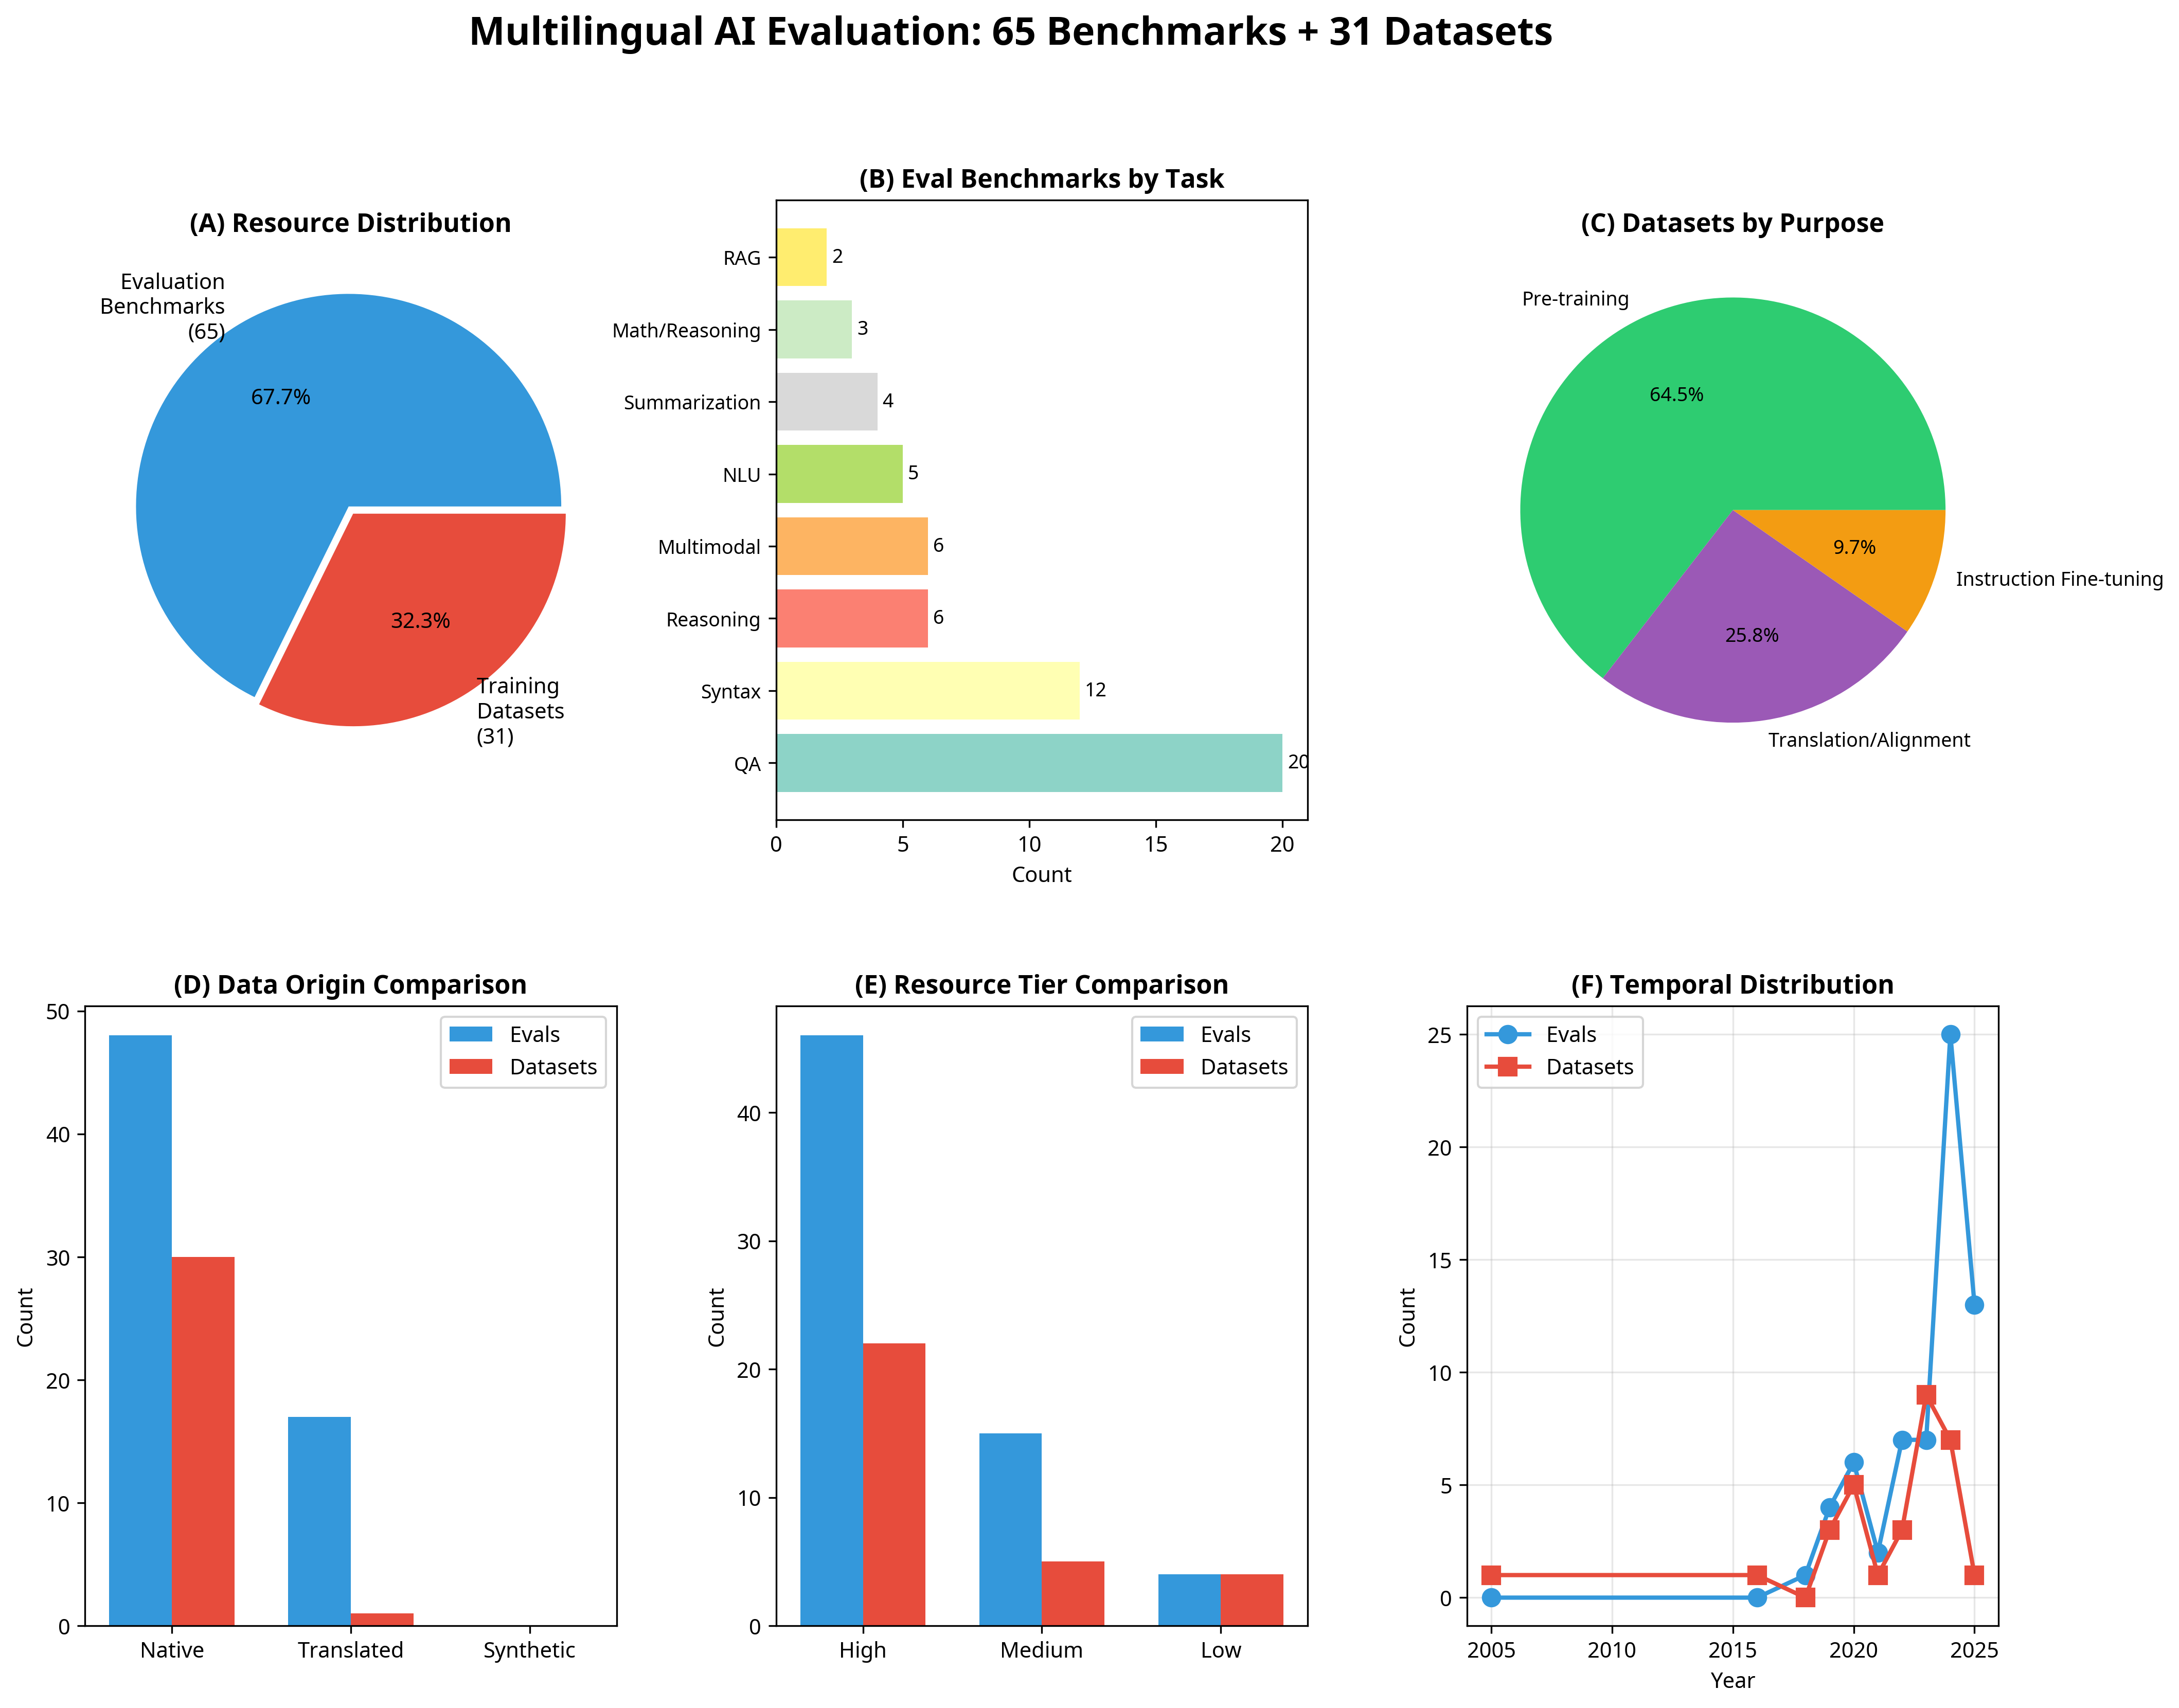
\includegraphics[width=0.8\linewidth]{images/figure_combined_overview.png}
%    \caption{Overview of the multilingual evaluation taxonomy comprising 65 evaluation benchmarks and 31 training datasets. (A) Resource distribution between benchmarks and datasets. (B) Evaluation benchmarks by task type. (C) Training datasets by purpose. (D) Data origin comparison. (E) Resource tier comparison. (F) Temporal distribution showing growth from 2018-2025.}
%    \label{fig:1_overview}
%\end{figure*}

\begin{figure*}[h!]
    \centering
    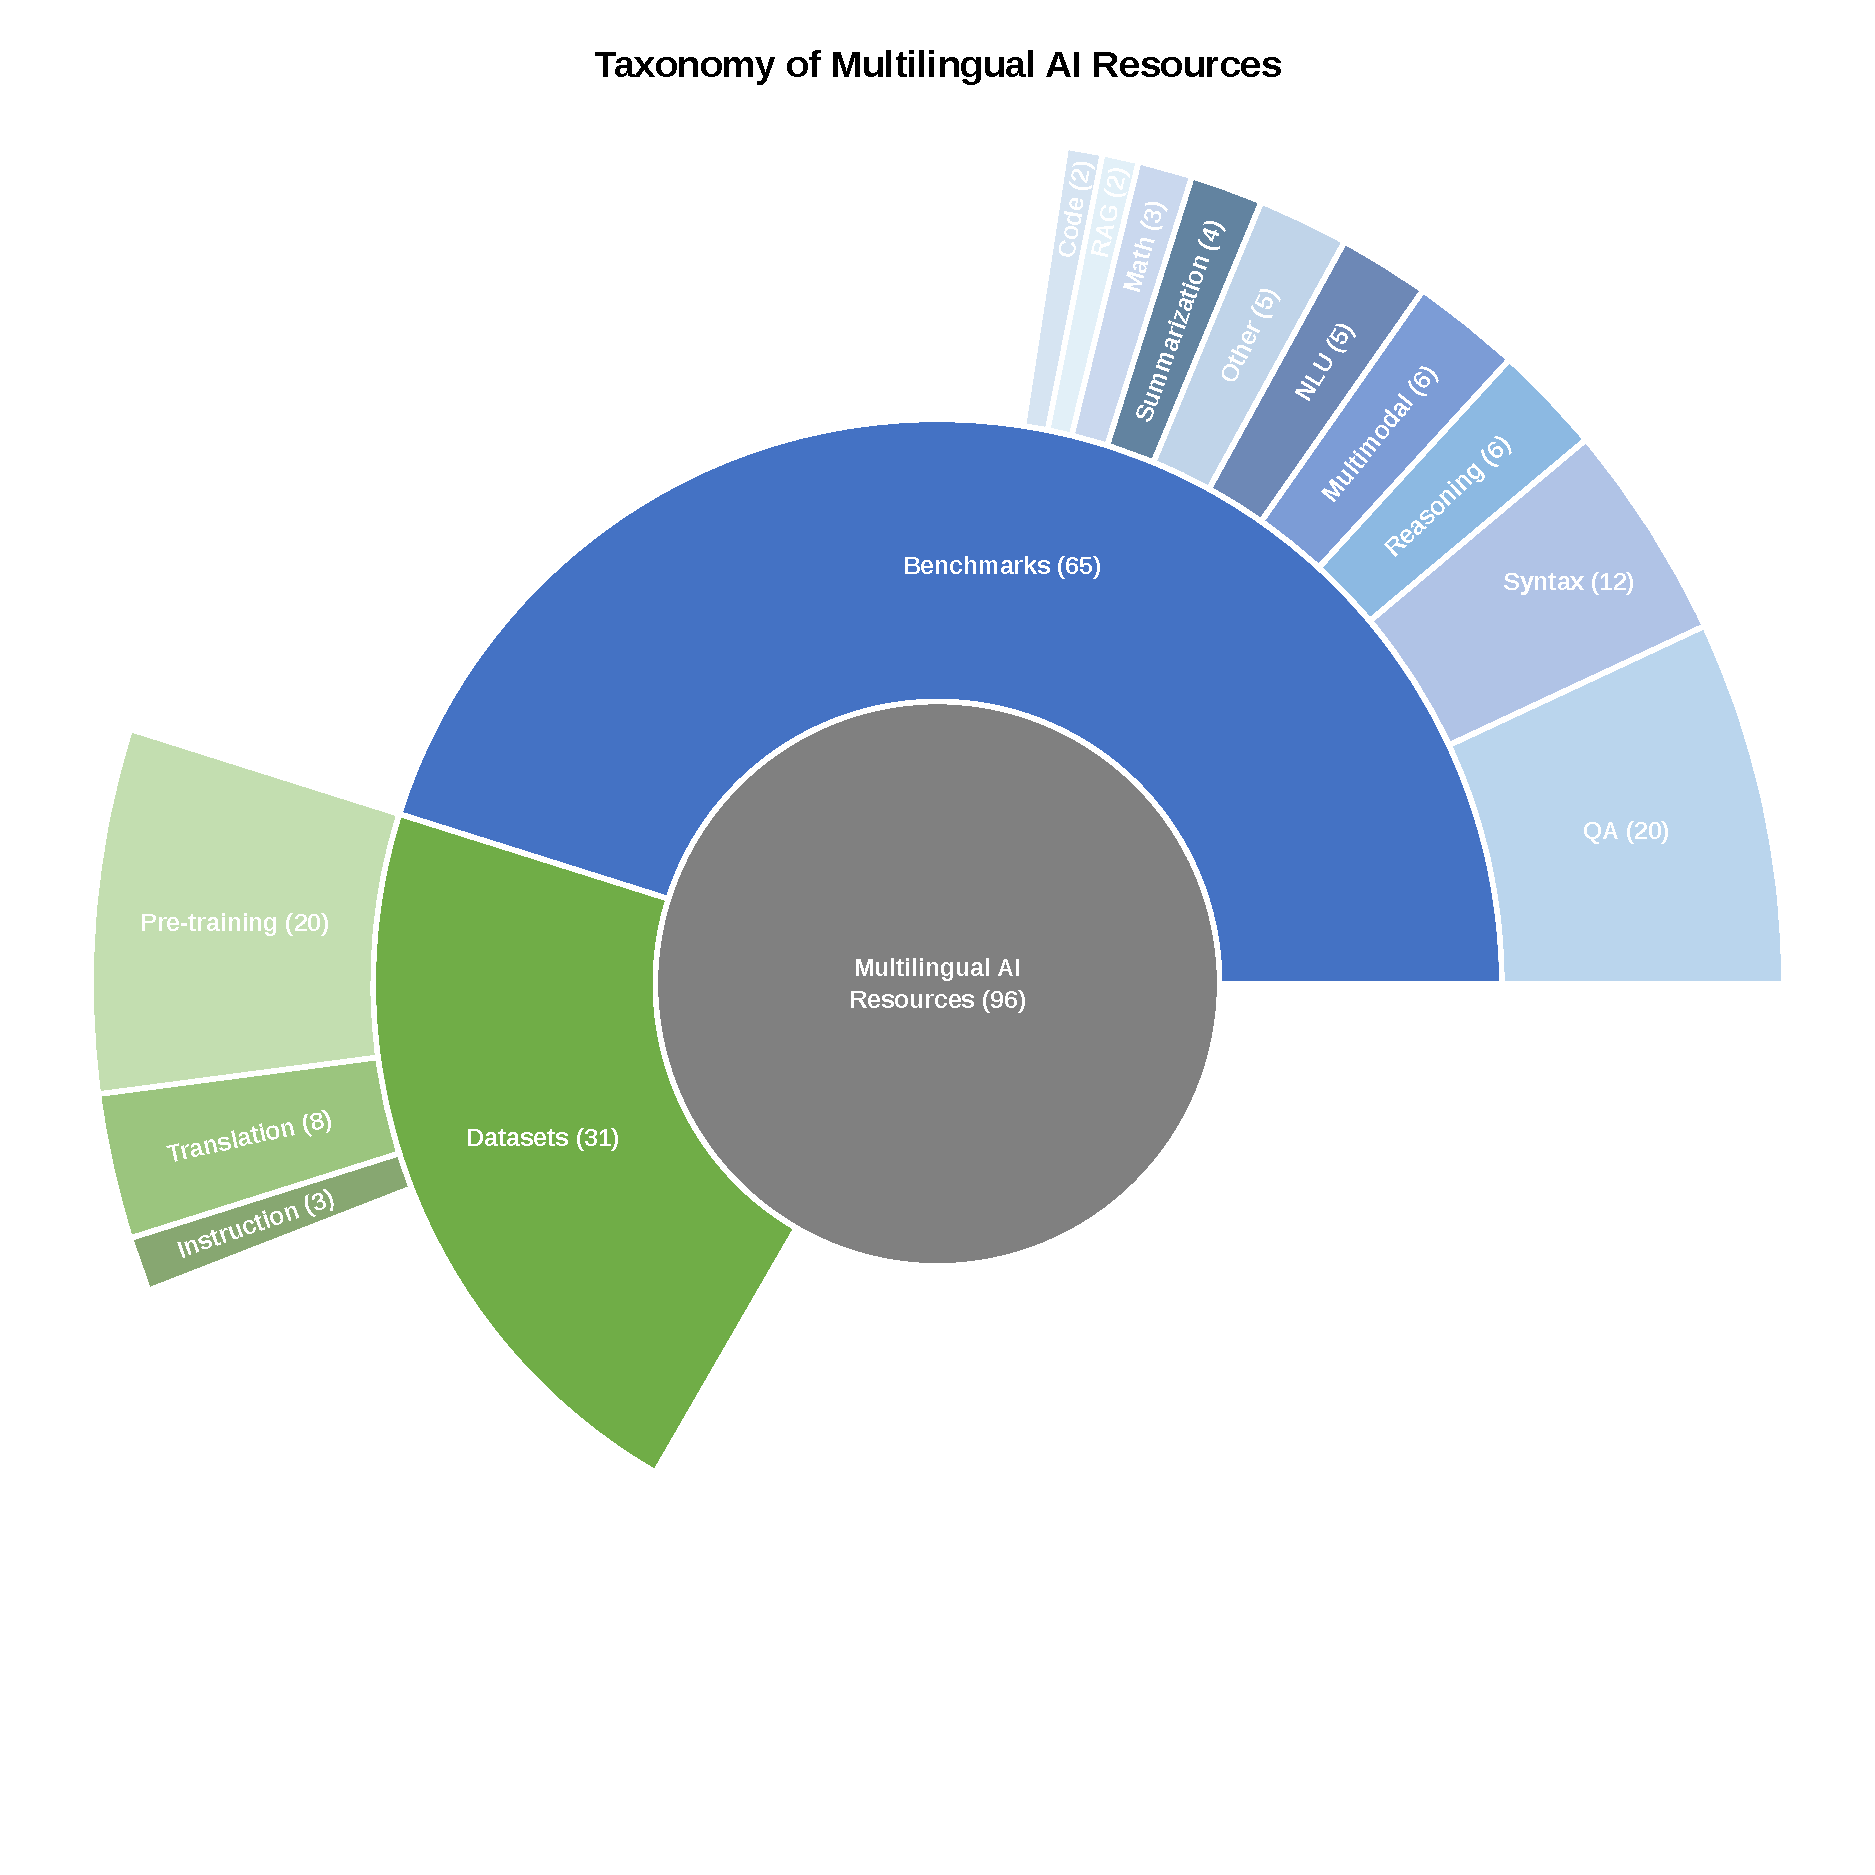
\includegraphics[width=0.8\linewidth]{images/taxonomy_sunburst_fixed.pdf}
    \caption{Sunburst visualization of the multilingual AI resource taxonomy. The center represents all 96 resources, with the inner ring dividing them into evaluation benchmarks (65, blue) and training datasets (31, green). The outer ring shows task class distribution for benchmarks (QA: 20, Syntax: 12, Reasoning: 6, Multimodal: 6, NLU: 5, and others) and primary purpose distribution for datasets (Pre-training: 20, Translation: 8, Instruction Fine-tuning: 3). Segment sizes are proportional to resource counts.}
    \label{fig:sunburst}
\end{figure*}


\begin{table*}[t]
\centering
\caption{Summary Statistics of Multilingual Evaluation Benchmarks and Training Datasets}
\label{tab:summary_stats}
\begin{tabular}{@{}lcc@{}}
\toprule
\textbf{Metric} & \textbf{Evaluation Benchmarks} & \textbf{Training Datasets} \\
\midrule
\textbf{Total Count} & 65 & 31 \\
\textbf{Unique Languages} & 139 & 139 \\
\textbf{Year Range} & 2018--2025 & 2005--2025 \\
\midrule
\multicolumn{3}{@{}l}{\textit{By Data Origin}} \\
\quad Native & 48 (73.8\%) & 23 (74.2\%) \\
\quad Translated & 17 (26.2\%) & 8 (25.8\%) \\
\midrule
\multicolumn{3}{@{}l}{\textit{By Resource Tier}} \\
\quad High & 46 (70.8\%) & 24 (77.4\%) \\
\quad Medium & 15 (23.1\%) & 5 (16.1\%) \\
\quad Low & 4 (6.2\%) & 2 (6.5\%) \\
\midrule
\multicolumn{3}{@{}l}{\textit{By Cultural Grounding}} \\
\quad Universal & 36 (55.4\%) & 22 (71.0\%) \\
\quad Culturally Anchored & 17 (26.2\%) & 6 (19.4\%) \\
\quad Region-Specific & 12 (18.5\%) & 3 (9.7\%) \\
\midrule
\multicolumn{3}{@{}l}{\textit{By Primary Purpose/Task}} \\
\quad QA & 20 (30.8\%) & -- \\
\quad Syntax & 12 (18.5\%) & -- \\
\quad Reasoning & 6 (9.2\%) & -- \\
\quad Multimodal & 6 (9.2\%) & -- \\
\quad Pre-training & -- & 20 (64.5\%) \\
\quad Translation/Alignment & -- & 8 (25.8\%) \\
\quad Instruction Fine-tuning & -- & 3 (9.7\%) \\
\bottomrule
\end{tabular}
\end{table*}




\section{Results}



\subsection{Datasets}

\begin{figure*}[t]
    \centering
    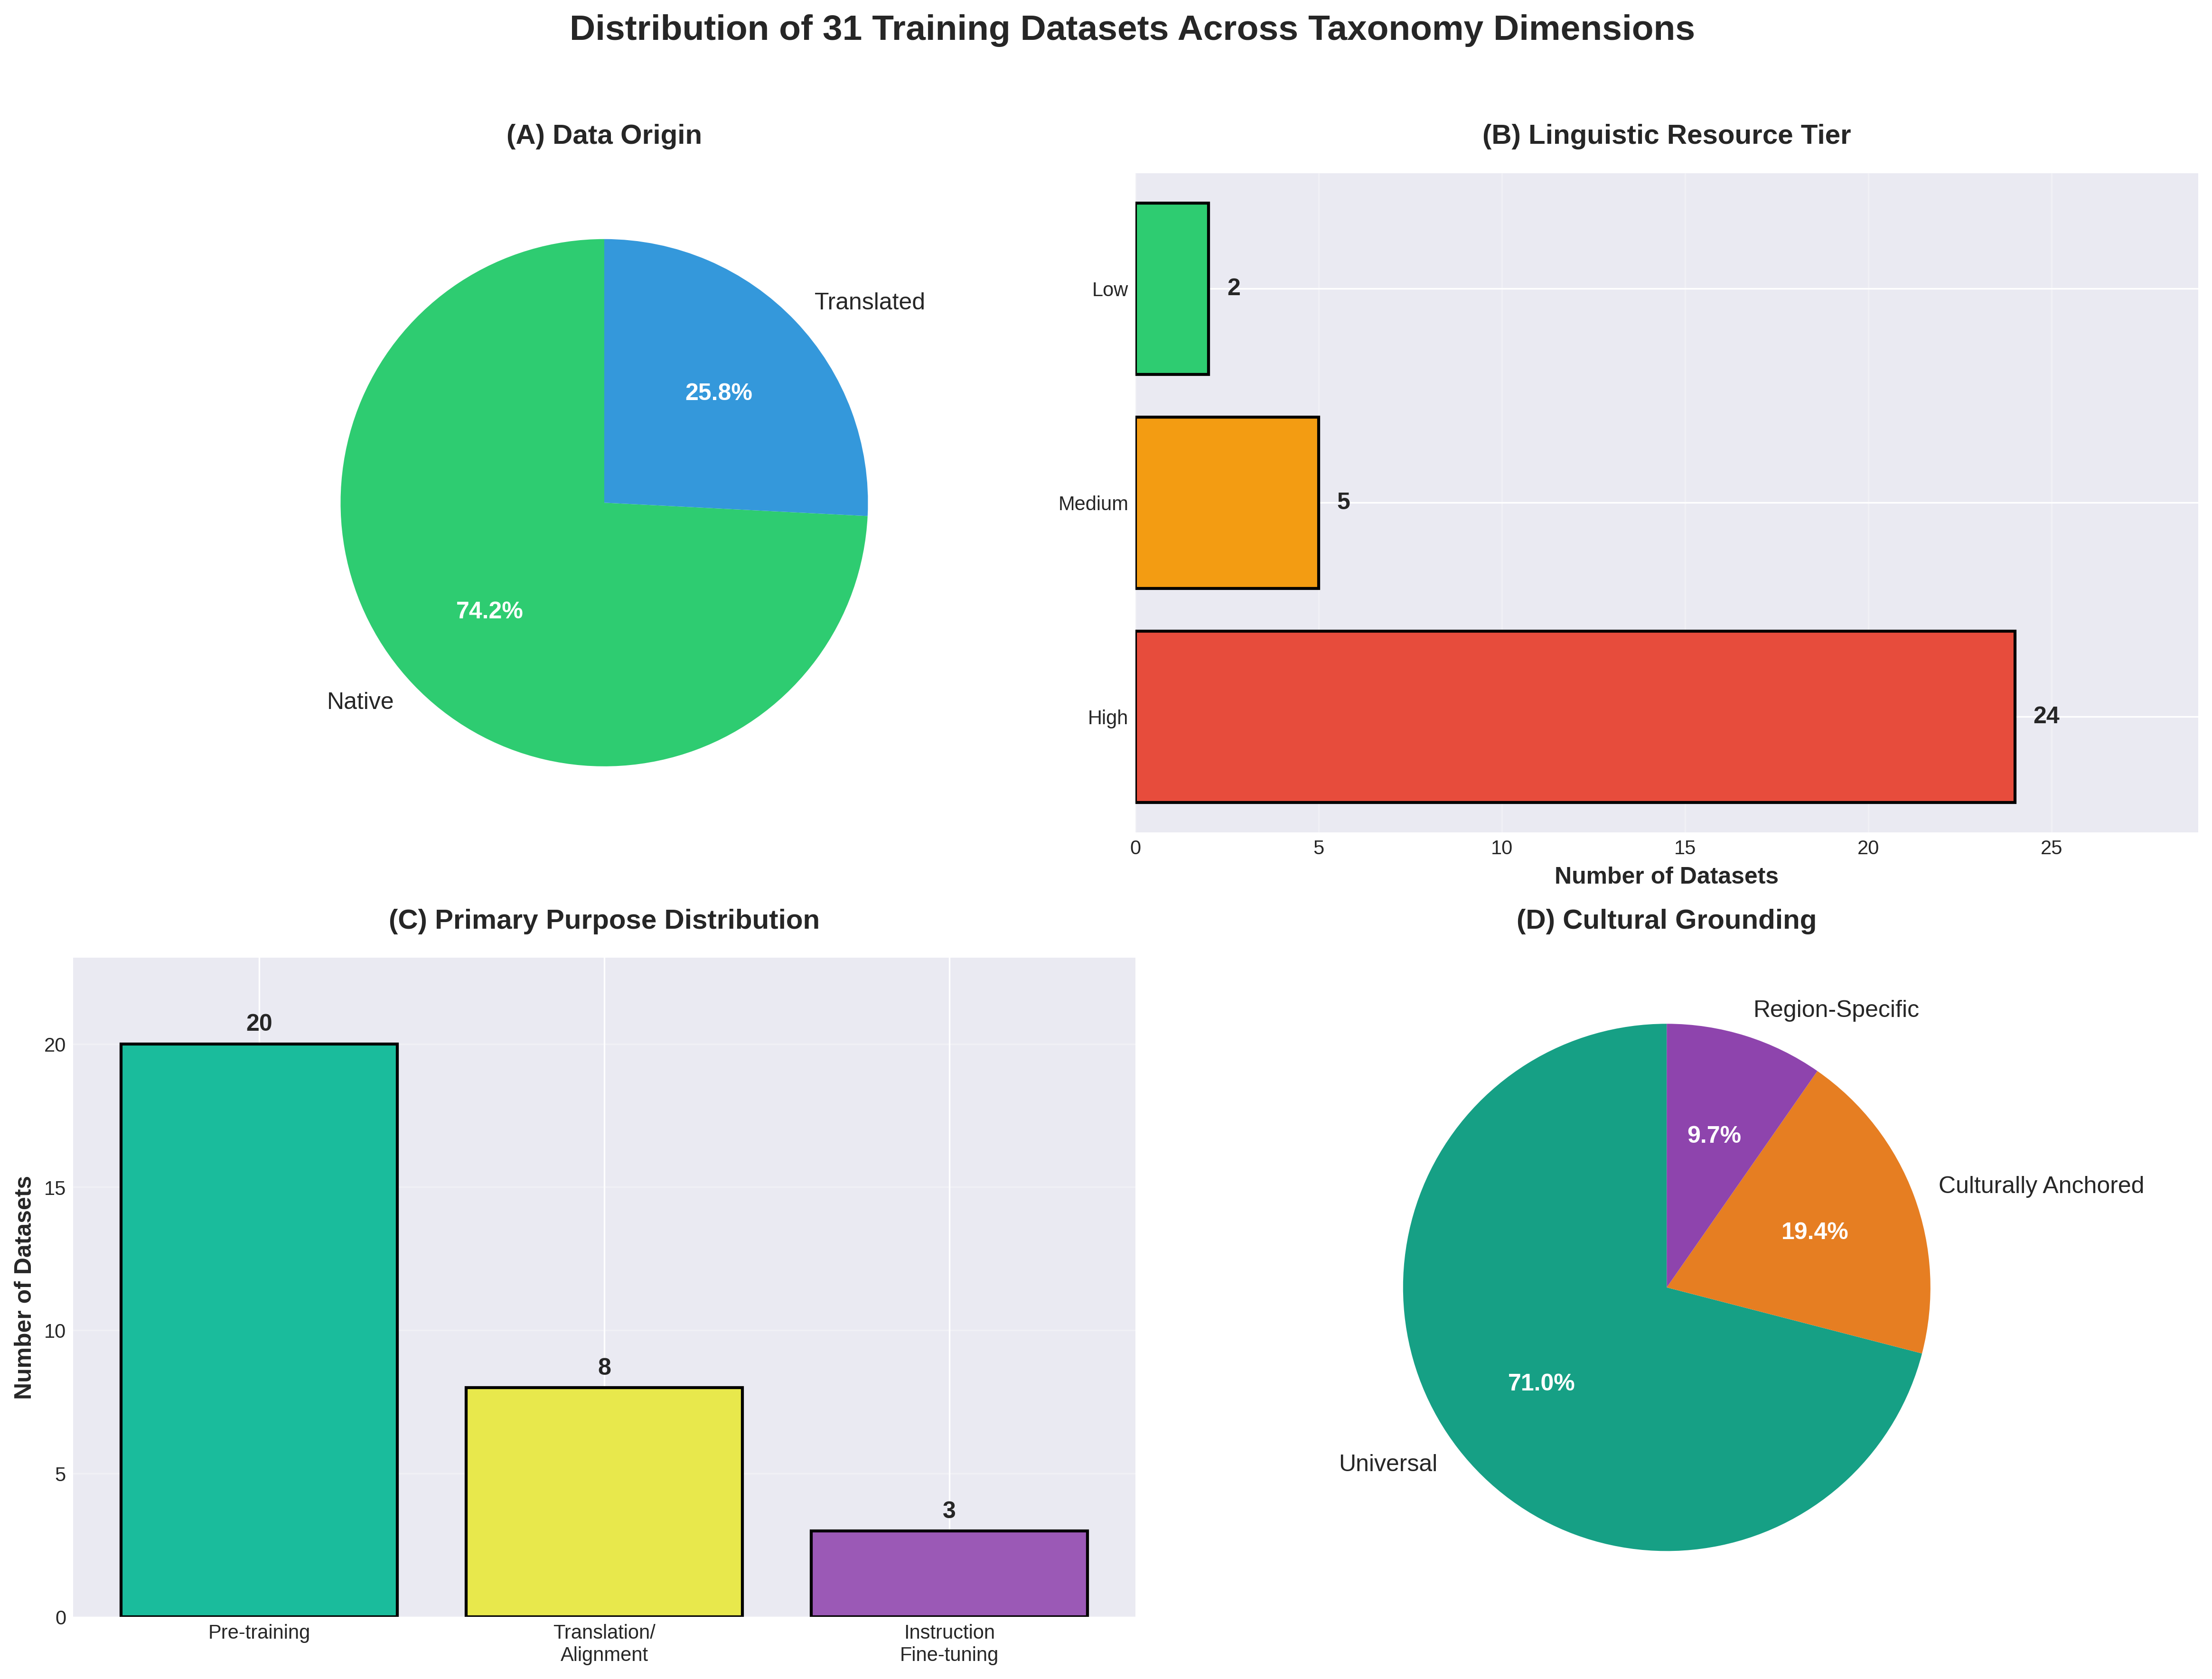
\includegraphics[width=0.8\linewidth]{images/dataset_distribution_figure.png}
    \caption{Distribution of 31 training datasets across taxonomy dimensions: (A) Data Origin, (B) Linguistic Resource Tier, (C) Primary Purpose, and (D) Cultural Grounding. High-resource languages and pre-training corpora dominate the dataset landscape.
}
    \label{fig:2_data_distribution}
\end{figure*}

\subsubsection{Pre-training Corpora}
\noindent
\citep{penedo2024finewebdatasetsdecantingweb} introduce FineWeb, a 15-trillion-token dataset derived from 96 Common Crawl snapshots, designed to produce high-performing LLMs. The authors address the lack of transparency in the creation of pre-training datasets for state-of-the-art open LLMs by carefully documenting and ablating their data curation process, including in-depth studies of deduplication and filtering strategies. They also release FineWeb-Edu, a 1.3-trillion-token subset of educational text filtered from FineWeb, which significantly improves model performance on knowledge and reasoning benchmarks. The authors have publicly released their data curation codebase and all models trained during their ablation experiments, advancing the community's understanding of how to create high-quality pre-training datasets.

\citep{messmer2025enhancingmultilingualllmpretraining} propose a model-based filtering framework for multilingual datasets to address the scarcity of research on non-English languages in this area. Their approach, which emphasizes transparency, simplicity, and efficiency, uses Transformer- and FastText-based classifiers to identify a diverse set of structured and knowledge-rich samples. The authors conduct comprehensive ablation studies on the FineWeb-2 dataset across various language families, scripts, and resource levels. They demonstrate that a 1B-parameter Llama model trained on a subset of the data selected by their method can match the MMLU score of a model trained on the full dataset with as little as 15\% of the tokens. The framework is extended to 20 languages, and the refined pre-training datasets are released to the public.

\citep{degibert2024newmassivemultilingualdataset} \citep{burchell2025expandedmassivemultilingualdataset}introduce the HPLT (High Performance Language Technologies) language resources, a massive multilingual dataset for training large-scale language models. The first version of the dataset includes a monolingual corpus of ~5.6 trillion tokens in 75 languages and an English-centric parallel corpus of 96 million sentence pairs across 18 language pairs. The second version significantly expands on the first, with a monolingual corpus of 8 trillion tokens in 193 languages and a parallel corpus of 380 million sentence pairs in 51 languages. The data is extracted from CommonCrawl and the Internet Archive, and the authors detail their open-source-based methods for data acquisition and processing. The HPLT resources are among the largest open text corpora ever released and have been shown to be valuable for training high-performing language models and machine translation systems.

\citep{raffel2023exploringlimitstransferlearning} introduce a unified framework for transfer learning in NLP that converts all text-based language problems into a text-to-text format. This allows for a systematic study of pre-training objectives, architectures, unlabeled datasets, and transfer approaches. The authors introduce the "Colossal Clean Crawled Corpus" (C4) and use it to train the Text-to-Text Transfer Transformer (T5) model. By combining their insights with scale, they achieve state-of-the-art results on a wide range of benchmarks, including summarization, question answering, and text classification. The authors released their dataset, pre-trained models, and code, which have become foundational for much of the subsequent work in the field.

 \citep{nguyen2023culturaxcleanedenormousmultilingual} present CulturaX, a 6.3-trillion-token multilingual dataset in 167 languages, created to address the lack of transparency and quality in training data for large language models. The dataset is built with a meticulous multi-stage cleaning and deduplication pipeline, including language identification, URL-based filtering, metric-based cleaning, document refinement, and data deduplication. CulturaX is designed to facilitate research into hallucination and bias in LLMs and to enable replication efforts. The dataset is fully released to the public on HuggingFace to promote advancements in multilingual LLMs.

 \citep{kudugunta2023madlad400multilingualdocumentlevellarge} introduce MADLAD-400, a manually audited, general-domain, 3-trillion-token monolingual dataset based on CommonCrawl, covering 419 languages. The authors discuss the limitations they discovered through the self-auditing process and the important role that data auditing played in the dataset's creation. Using this dataset and other publicly available data, they trained a 10.7B-parameter multilingual machine translation model covering over 450 languages, which they found to be competitive with much larger models. They also trained an 8B-parameter language model and evaluated its few-shot translation capabilities. The baseline models are released to the research community.

  \citep{weber2024redpajamaopendatasettraining} introduce RedPajama, a large-scale open dataset for training language models, created to address the lack of transparency in dataset curation from prominent models. The authors release two datasets: RedPajama-V1, an open reproduction of the LLaMA training dataset, and RedPajama-V2, a massive web-only dataset of over 100 trillion tokens with quality signals and metadata. The work addresses three key challenges in open-source model development: transparency in data curation, access to high-quality data, and availability of artifacts for analysis. The authors demonstrate the effectiveness of their dataset by conducting ablation studies with models up to 1.6B parameters, showing that the quality signals can be used to curate high-quality subsets. The RedPajama datasets have been used to train several production models, including Snowflake Arctic and Salesforce XGen, highlighting their value to the community and advancing the development of transparent and high-performing language models.

  \citep{Gokaslan2019OpenWeb} introduce OpenWebText, an open-source replication of OpenAI's WebText dataset used to train GPT-2. The corpus was created by extracting URLs from the Reddit submissions dataset, which were then deduplicated and filtered to exclude non-HTML content. Web pages were downloaded in parallel and extracted using the newspaper Python package, with non-English content filtered out using Facebook FastText. Near-duplicate documents were identified using local-sensitivity hashing (LSH) with 5-gram sets, removing documents with similarity >0.5. Documents with fewer than 128 tokens were also removed. The final corpus contains 38GB of text data from 8,013,769 documents, providing a publicly available alternative to OpenAI's proprietary WebText for training and evaluating large language models. The dataset is released under a Creative Commons CC0 license and has become a widely-used resource for pre-training language models in the research community.

  \citep{ortiz-suarez-etal-2020-monolingual} investigate a monolingual approach for building contextualized word embeddings for mid-resource languages, using the large, multilingual OSCAR corpus extracted from Common Crawl. The authors train monolingual ELMo embeddings for five languages and evaluate them on part-of-speech tagging and parsing tasks. They demonstrate that despite the noisy nature of the web-crawled data, embeddings trained on the larger and more diverse OSCAR corpus significantly outperform those trained on the smaller, cleaner Wikipedia corpus. Furthermore, the OSCAR-based ELMo embeddings establish a new state of the art for all five languages, even surpassing the performance of multilingual models like BERT. This work shows that for mid-resource languages, the scale and diversity of a large monolingual corpus can be more beneficial than the cross-lingual knowledge transfer in multilingual models, underscoring the value of web-scale data for improving monolingual representations.
  
\begin{table}[htbp]
\centering
\caption{Distribution of Training Datasets by Primary Purpose}
\label{tab:dataset-purpose}
\begin{tabular}{lcc}
\toprule
\textbf{Primary Purpose} & \textbf{Count} & \textbf{Percentage} \\
\midrule
Pre-training Corpora & 20 & 64.5\% \\
Translation/Alignment & 8 & 25.8\% \\
Instruction Fine-tuning & 3 & 9.7\% \\
\midrule
\textbf{Total} & \textbf{31} & \textbf{100.0\%} \\
\bottomrule
\end{tabular}
\end{table}

\citep{langlais2025commoncorpuslargestcollection} introduce Common Corpus, the largest open dataset for language model pre-training, containing approximately two trillion tokens. The dataset is designed to be compliant with AI legislation and data security regulations by including only uncopyrighted or permissibly licensed content. It features a wide variety of languages, from major European languages to low-resource ones, and includes a significant amount of code. The authors provide a detailed account of the data assembly, filtering, and curation process. Common Corpus is already in use by industry leaders and is intended to be a critical infrastructure for open science research in LLMs, addressing the need for a large-scale, ethically sourced pre-training dataset.

\citep{laurençon2023bigsciencerootscorpus16tb} document the creation of the Responsible Open-science Open-collaboration Text Sources (ROOTS) corpus, a 1.6TB dataset spanning 59 languages. This work was part of the BigScience workshop, a year-long international and multidisciplinary initiative focused on the ethical and responsible research and training of large language models. The ROOTS corpus was used to train the 176-billion-parameter BigScience Large Open-science Open-access Multilingual (BLOOM) language model. The authors have released a large subset of the corpus, along with the processing tools used to create it, to empower large-scale monolingual and multilingual modeling projects and to stimulate further research on this large multilingual resource.

\citep{kakwani-etal-2020-indicnlpsuite} \citep{doddapaneni2023leavingindiclanguagebehind} present a series of resources for developing Natural Language Understanding (NLU) capabilities for Indian languages. The first version, IndicNLPSuite, introduced monolingual corpora for 11 major Indian languages (8.8 billion tokens), pre-trained word embeddings (FastText), pre-trained language models (ALBERT), and the IndicGLUE benchmark. The second version significantly expands on this with IndicCorp, the largest monolingual corpora for Indian languages with 20.9 billion tokens covering 24 languages. This work also introduces IndicXTREME, a human-supervised benchmark for nine NLU tasks across 20 languages, and IndicBERT v2, a state-of-the-art model that shows a 2-point improvement over strong baselines. These resources are a major contribution to the field and are publicly available.




 \citep{Khan_2024} present IndicLLMSuite, a comprehensive suite of resources for building LLMs for 22 Indian languages. The suite includes a 251-billion-token pre-training corpus and a 74.8-million-pair instruction-tuning dataset. The authors developed a robust, open-source pipeline for curating data from diverse sources like websites, PDFs, and videos, incorporating best practices for cleaning and deduplication. The instruction-tuning data was created by combining existing Indic datasets, translating and transliterating English datasets, and generating synthetic conversations using LLaMa2 and Mixtral models. The work also addresses toxicity alignment by creating a dataset of toxic prompts and non-toxic responses. IndicLLMSuite provides a blueprint for creating similar resources for other language families and is released with permissive licenses to foster research and development in Indic LLMs.

 \citep{kummervold-etal-2022-norwegian} introduce the Norwegian Colossal Corpus (NCC), a 49GB corpus of clean Norwegian text containing over 7 billion words. The NCC was created to address the lack of sufficient data for training high-quality Norwegian language models. It is composed of a wide variety of sources, including books, newspapers, government documents, and public reports, and covers both Norwegian Bokmål and Norwegian Nynorsk. Each document is tagged with metadata to allow for the creation of specific sub-corpora. The corpus is openly available to foster the development of better Norwegian and multilingual language models.
 
\citep{ng2025sealionsoutheastasianlanguages} introduce the SEA-LION family of models, which are designed to address the under-representation of Southeast Asian (SEA) languages in LLMs. The models, Llama-SEA-LION-v3-8B-IT and Gemma-SEA-LION-v3-9B-IT, support 11 SEA languages. The authors use large-scale multilingual continued pre-training and a comprehensive post-training regime that includes multiple stages of instruction fine-tuning, alignment, and model merging. The SEA-LION models achieve state-of-the-art performance on multilingual benchmarks for SEA languages and are open-sourced to benefit the wider community. This work is associated with the SEA-PILE dataset, which contains 120 billion tokens.

 \citep{thapa2025developmentpretrainedtransformerbasedmodels} present pre-trained transformer models for Nepali, a low-resource language spoken by 32 million people. The authors compiled a 27.5 GB corpus by scraping 99 Nepali news websites—2.4 times larger than previous corpora—and pre-trained three models: BERT (110M parameters), RoBERTa (125M), and GPT-2 (124M). After preprocessing with deduplication, language filtering, and Unicode normalization, they trained encoder models using masked language modeling for 400k steps and a decoder model using causal language modeling for 500k steps. On the Nep-gLUE benchmark (comprising NER, POS tagging, text classification, and sentence similarity), their RoBERTa achieved 95.60, outperforming the previous best by 2 points. For text generation, their instruction-tuned GPT-2 achieved ROUGE-L of 17.76 on summarization, demonstrating improvements in both understanding and generation. This work addresses the gap in decoder-based architectures for Nepali and establishes new state-of-the-art results, providing a foundation for future low-resource NLP research.

  \citep{tran2024uccixirishexcellencelargelanguage} presents the first large-scale, open-source Irish language model specifically designed for an extremely low-resource linguistic setting. Built upon Llama 2-13B, UCCIX introduces an efficient continued pre-training framework that adapts large language models to low-resource contexts using only hundreds of millions of Irish tokens—far below standard data requirements prescribed by scaling laws. The authors construct a 1.8 billion-character corpus from multiple Irish text sources, apply a staged adaptation strategy beginning with parallel English-Irish data to facilitate linguistic transfer, and expand the model’s tokenizer with 10 000 Irish-specific tokens to improve fluency and generation speed. Following supervised instruction fine-tuning, the resulting model, UCCIX-Instruct, demonstrates state-of-the-art performance across Irish benchmarks, surpassing much larger models such as Llama 2-70B and BLOOM-7B by up to 12\% on key tasks. To support systematic evaluation, the authors also release two new datasets—IrishQA, a culturally grounded question-answering benchmark, and an Irish-translated MT-bench for instruction-following assessment. While UCCIX achieves near GPT-3.5 performance on Irish MT-bench despite being more than ten times smaller, the authors note partial catastrophic forgetting of English capabilities. Overall, the work provides a methodological and empirical foundation for extending large language models to endangered and low-resource languages, emphasizing both linguistic preservation and digital inclusivity.

\citep{adebara2023serengetimassivelymultilinguallanguage} introduce SERENGETI, a massively multilingual language model that covers 517 African languages and language varieties, significantly expanding the linguistic coverage of existing models, which only include about 31 of the ~2,000 African languages. The authors evaluate their models on eight natural language understanding tasks across 20 datasets and show that SERENGETI outperforms other models on 11 of these datasets, achieving an average F1 score of 82.27. The paper also includes an analysis of model errors to investigate the influence of language genealogy and linguistic similarity in zero-shot settings. The models are publicly available for research.

\citep{oladipo-etal-2023-better} highlight the importance of data quality in pre-training multilingual language models, particularly for low-resource languages. The authors introduce a new multilingual pre-training corpus for 16 African languages, created by carefully auditing and cleaning existing web-crawled data from sources like mC4. They then pre-train a new T5-based model on this higher-quality dataset and demonstrate its superior performance on four downstream NLP tasks compared to existing pre-trained models. Notably, on a cross-lingual QA evaluation, their new model is more than twice as effective as multilingual T5. This work underscores the critical role of data quality in pre-training, and all code, data, and models are publicly available.

\begin{figure*}[t]
    \centering
    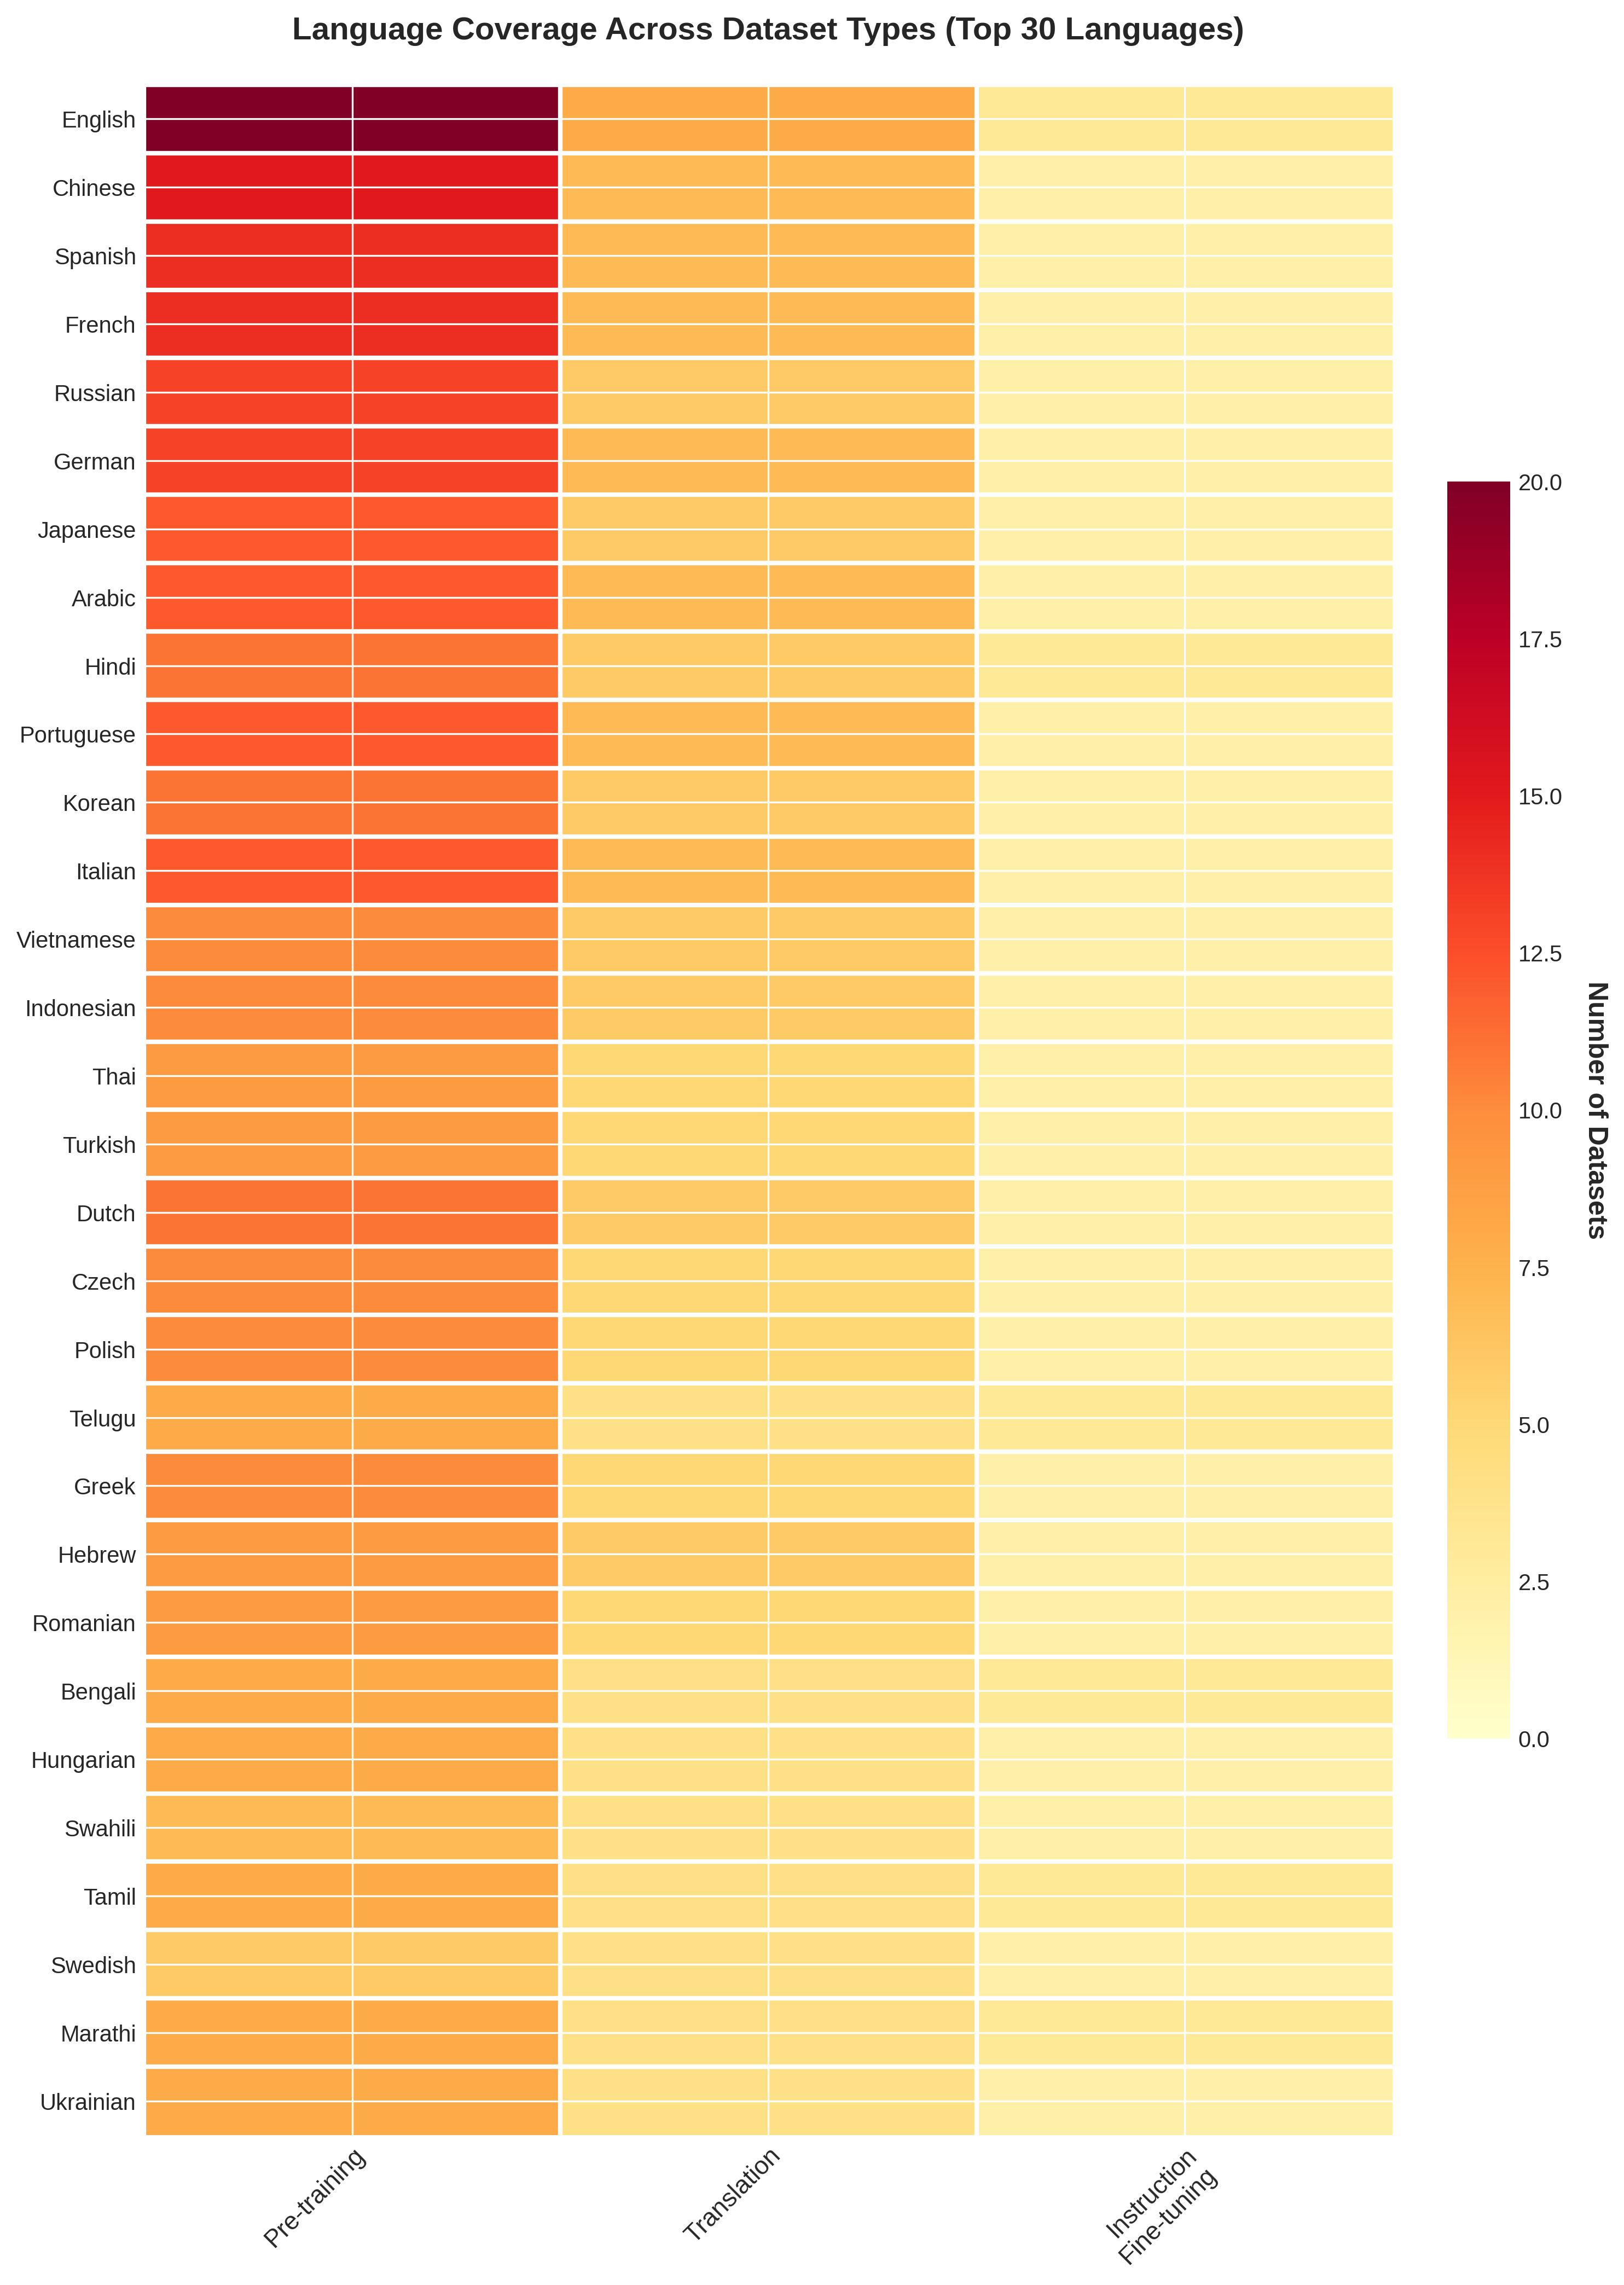
\includegraphics[width=0.8\linewidth]{images/dataset_language_heatmap.png}
    \caption{Language coverage heatmap showing the number of datasets supporting each of the top 30 languages across three dataset types. Color intensity indicates coverage depth, with English showing universal coverage while low-resource languages remain underrepresented.}
    \label{fig:language_heatmap}
\end{figure*}


\subsubsection{Translation/Alignment Corpora}
\noindent

 \citep{schwenk2020ccmatrixminingbillionshighquality} present CCMatrix, a massive parallel corpus created by applying margin-based bitext mining to billions of sentences from the Common Crawl. Using a unified approach for 38 languages, they mined 4.5 billion parallel sentences, with 661 million aligned with English. The authors demonstrate the quality of the mined bitexts by training NMT systems for most language pairs and evaluating them on standard test sets (TED, WMT, WAT). Notably, their systems, trained only on the mined data, achieved new state-of-the-art results on the WMT’19 test set for English-German, English-Russian, and English-Chinese, outperforming the best single systems by a significant margin. This work showcases the effectiveness of large-scale bitext mining from web data for training high-quality machine translation systems, even for distant language pairs.

  \citep{el-kishky-etal-2020-ccaligned} introduce CCAligned, a dataset of cross-lingual web-document pairs created by exploiting signals embedded in URLs. By mining 68 snapshots of the Common Crawl, they identified over 392 million URL pairs across 8,144 language pairs (137 involving English) that are translations of each other, with an average precision of 94.5\%. The authors also provide baseline methods for identifying aligned documents based on textual content using cross-lingual representations. They demonstrate the value of this dataset by using it to mine parallel sentences and training machine translation models that achieve strong performance. CCAligned is a valuable resource for fostering research in cross-lingual NLP, especially for low- and medium-resource languages.

   \citep{banon-etal-2020-paracrawl} describe the ParaCrawl project, an effort to create the largest publicly available parallel corpora by crawling the web. The paper details the open-source software and methods used for this web-scale acquisition of parallel data. The authors empirically compare different methods for sentence alignment and filtering, and release benchmark datasets for these tasks. They also describe the released parallel corpora and evaluate their quality and usefulness for training machine translation systems. ParaCrawl has become a key resource for the machine translation community, providing large-scale parallel data for a wide range of languages.

   \citep{schwenk-etal-2021-wikimatrix} present WikiMatrix, a parallel corpus created by mining parallel sentences from Wikipedia articles in 96 languages. Using an approach based on multilingual sentence embeddings, they extracted 135 million parallel sentences for 1,620 language pairs. A key feature of WikiMatrix is that it does not limit extraction to alignments with English, resulting in a large number of direct alignments between non-English languages (only 34 million of the 135 million sentences are aligned with English). The authors demonstrate the quality of the corpus by training NMT systems for 1,886 language pairs and evaluating them on the TED corpus, achieving strong BLEU scores. WikiMatrix is particularly valuable for training MT systems between distant languages without pivoting through English.



   \citep{koehn-2005-europarl} introduces the Europarl corpus, a parallel corpus of 11 languages collected from the proceedings of the European Parliament. This corpus, one of the first large-scale, publicly available parallel corpora, has been a foundational resource for the statistical machine translation (SMT) community. The paper describes the acquisition of the corpus and its application as training data for SMT systems. The authors trained SMT systems for 110 language pairs, providing insights into the challenges of multilingual machine translation at the time. Europarl has been instrumental in the development and evaluation of machine translation systems and remains a valuable resource for NLP research.

\citep{lison-etal-2018-opensubtitles2018} present a method for improving sentence alignments in the OpenSubtitles corpus, a large and noisy parallel corpus derived from movie and TV subtitles. The authors address the challenges of aligning sentences in such noisy data by using a statistical rescoring method. The OpenSubtitles corpus is a widely used resource in multilingual NLP, providing parallel data for a vast number of language pairs. This work on improving the quality of sentence alignments in OpenSubtitles2018 enhances its value as a resource for training and evaluating machine translation and other cross-lingual models.

\citep{tiedemann-2020-tatoeba} describes the development of a new benchmark for machine translation that provides training and test data for thousands of language pairs covering over 500 languages. The Tatoeba Translation Challenge aims to spur the development of open translation tools and models with much broader language coverage. The benchmark provides realistic low-resource scenarios, a comprehensive collection of diverse datasets with systematic language and script annotation, and data splits that extend the coverage of existing benchmarks. The release also includes a growing number of pre-trained baseline models.


\subsubsection{Instruction Fine-tuning Datasets }
\noindent

 \citep{singh2024ayadatasetopenaccesscollection} introduce the Aya Dataset, a large-scale, human-curated instruction-following dataset designed to bridge the language gap in instruction fine-tuning resources. The authors worked with fluent speakers from around the world to collect natural instances of instructions and completions in 65 languages. In addition to the human-curated data, they created the Aya Collection, a massive collection of 513 million instances generated by templating and translating existing datasets across 114 languages. The initiative also produced the Aya Annotation Platform and the Aya Evaluation Suite. This work is a significant contribution to multilingual NLP, providing a valuable resource for training and evaluating models in a wide range of languages and serving as a model for participatory research.
 
\citep{li2023bactrianxmultilingualreplicableinstructionfollowing} present Bactrian-X, a comprehensive multilingual parallel dataset of 3.4 million instruction-response pairs across 52 languages, created to address the scarcity of high-quality multilingual instruction-tuning data. Using this dataset, the authors train a set of lightweight adapters with Low-Rank Adaptation (LoRA). These adapters can be easily integrated with large language models as plug-ins for different languages or language groups. The authors show that models using these adapters outperform both the vanilla models and existing instruction-tuned models in various multilingual evaluation settings. The code and models are publicly available.

\citep{muennighoff2023crosslingualgeneralizationmultitaskfinetuning} investigate the use of multitask prompted finetuning (MTF) to improve the crosslingual generalization of large language models. The authors apply MTF to the multilingual BLOOM and mT5 models, creating the finetuned variants BLOOMZ and mT0. They find that finetuning on English tasks with English prompts enables generalization to non-English languages, and that finetuning on multilingual tasks with English prompts further improves performance. The authors also introduce xP3, a composite of supervised datasets in 46 languages with both English and machine-translated prompts. Their findings suggest that models can learn task- and language-agnostic capabilities, and they have released their code, datasets, and models to the public.



\begin{figure*}[t]
    \centering
    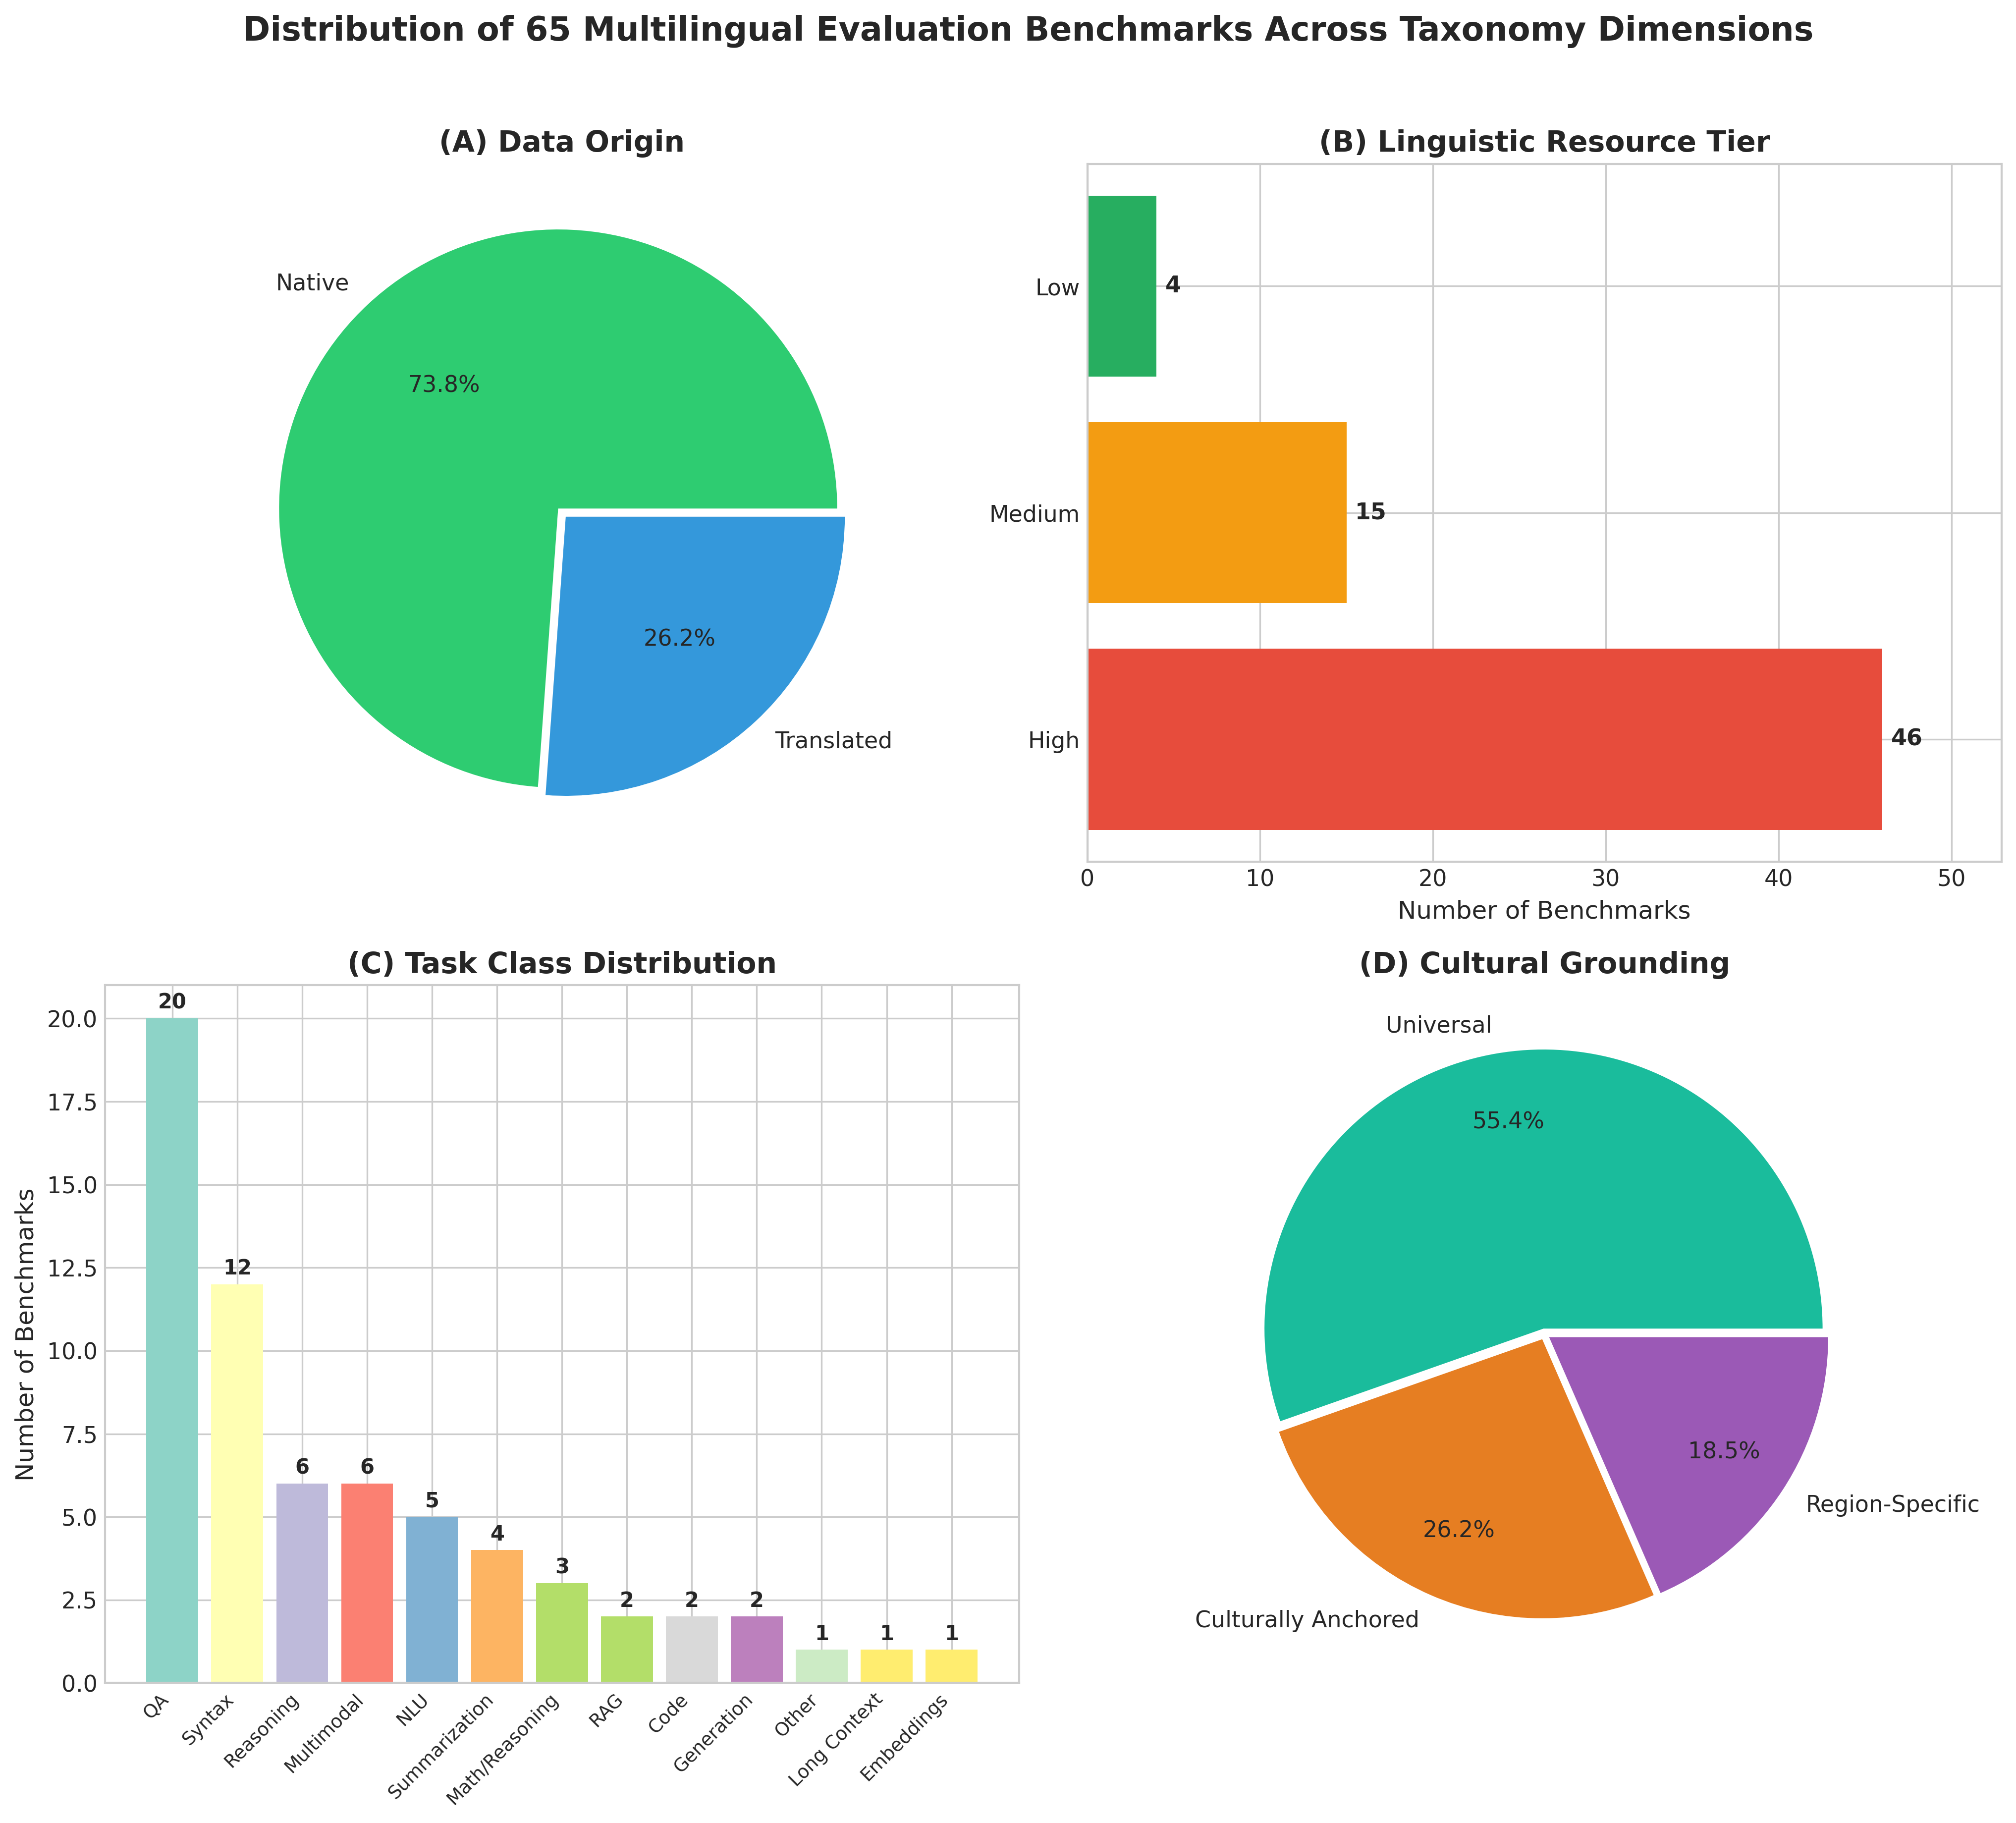
\includegraphics[width=0.8\linewidth]{images/figure4_distribution_complete.png}
    \caption{Distribution of 65 multilingual evaluation benchmarks across taxonomy dimensions. (A) Data origin: 73.8\% native vs 26.2\% translated. (B) Linguistic resource tier distribution. (C) Task class distribution showing QA (20) and Syntax (12) as dominant categories. (D) Cultural grounding with 55.4\% universal benchmarks.}
    \label{fig:2_distribution}
\end{figure*}

% Table 3: Top 20 Languages by Benchmark Coverage
\begin{table}[t]
\centering
\caption{Top 20 Languages by Benchmark Coverage}
\label{tab:languages}
\begin{tabular}{@{}clr|clr@{}}
\toprule
\textbf{Rank} & \textbf{Language} & \textbf{Count} & \textbf{Rank} & \textbf{Language} & \textbf{Count} \\
\midrule
1 & English & 37 & 11 & Korean & 26 \\
2 & Chinese & 35 & 12 & Italian & 25 \\
3 & Spanish & 31 & 13 & Vietnamese & 24 \\
4 & German & 30 & 14 & Thai & 23 \\
5 & French & 30 & 15 & Indonesian & 23 \\
6 & Russian & 30 & 16 & Turkish & 18 \\
7 & Arabic & 28 & 17 & Dutch & 18 \\
8 & Japanese & 28 & 18 & Czech & 15 \\
9 & Hindi & 27 & 19 & Polish & 14 \\
10 & Portuguese & 27 & 20 & Greek & 13 \\
\bottomrule
\end{tabular}
\end{table}

\subsection{Evals/Benchmarks}

\subsubsection{Question Answering (QA}
\noindent

\citep{Artetxe_2020} present XQuAD and MONOTRANS, studying cross-lingual transfer of monolingual transformer models. MONOTRANS transfers a monolingual masked language model to new languages by learning new embedding matrices while freezing the transformer body, without shared vocabularies or joint multilingual training, and is evaluated against joint multilingual (JOINTMULTI), joint bilingual (JOINTPAIR), and cross-lingual embedding (CLWE) models on XNLI, MLDoc, PAWS-X, and XQuAD. XQuAD contains 240 context paragraphs and 1,190 question-answer pairs from SQuAD v1.1, professionally translated into ten languages (Spanish, German, Greek, Russian, Turkish, Arabic, Vietnamese, Thai, Chinese, Hindi), with consistent translation of questions and transliteration of named entities. Results show MONOTRANS is competitive with multilingual models, with semantic knowledge transferring across languages while syntactic structures remain challenging; larger vocabulary sizes, adapters, and language-specific position embeddings further improve performance. These findings challenge the need for shared vocabularies or joint training for cross-lingual generalization, highlighting the transferability of deep monolingual representations and establishing XQuAD as a comprehensive benchmark for cross-lingual QA.

\citep{lewis2019mlqa} present MLQA, a multi-way aligned benchmark for evaluating cross-lingual extractive question answering models across seven diverse languages. While question answering (QA) models have progressed rapidly in English, the lack of large, high-quality, and parallel evaluation datasets in other languages has made it difficult to train and rigorously measure the performance of multilingual QA systems. To address this, the authors created a large-scale dataset with over 12,000 instances in English and over 5,000 in each of six other languages (Arabic, German, Spanish, Hindi, Vietnamese, and Simplified Chinese), where each instance is parallel across four languages on average. They introduce a novel annotation pipeline that first automatically identifies parallel sentences in Wikipedia articles, then uses crowd-workers to create English question-answer pairs tied to those sentences, and finally employs professional translators to translate the questions and annotate answers in the target languages. Evaluations of state-of-the-art cross-lingual models, along with machine-translation baselines, demonstrate that performance when transferring to other languages is significantly behind the training-language (English) performance. The key strength of this work lies in providing the community with a high-quality, large-scale, and highly parallel evaluation benchmark that enables fairer comparisons across languages, introduces novel evaluation tasks like generalized cross-lingual transfer, and establishes a crucial tool to spur research in multilingual QA.

\citep{bandarkar2023belebele} present BELEBELE, a large-scale, parallel machine reading comprehension benchmark designed to rigorously evaluate text models across 122 language variants. While multilingual models are increasingly common, prior evaluations have been hindered by a lack of high-coverage, parallel benchmarks, with most existing datasets focusing on fewer than 30 high- or medium-resource languages. To address this, the authors created a new dataset consisting of 900 multiple-choice questions, each based on a short passage from the FLORES-200 dataset and translated by human experts to ensure direct comparability across all languages. They introduce a carefully curated set of questions with strong negative answers designed to challenge state-of-the-art models and punish simple pattern-matching heuristics, while remaining solvable by humans with near-perfect accuracy. The benchmark's questions often require understanding multiple sentences but do not necessitate external knowledge or complex reasoning. Results demonstrate that while large, English-centric LLMs show surprising cross-lingual generalization, smaller masked language models (MLMs) pretrained on balanced multilingual data still understand a far greater number of languages. The key strength of this work lies in providing the community with a massive, parallel, and high-quality evaluation suite that enables a clearer and more direct comparison of the multilingual comprehension capabilities of NLP systems across an unprecedented number of diverse languages.

\citep{singh2024indic} present the Indic-QA Benchmark, a large-scale, multilingual dataset designed to rigorously evaluate the context-grounded question-answering capabilities of Large Language Models (LLMs) across 11 major Indian languages. While LLMs excel in English, their performance in low-resource languages remains underexplored due to a lack of high-quality, large, and domain-diverse evaluation benchmarks. To address this gap, the authors constructed the largest publicly available CQA dataset for 11 Indic languages by compiling existing datasets, translating several major English QA benchmarks, and generating a new synthetic dataset with manual verification. The benchmark covers both extractive and abstractive QA tasks and was developed with a focus on cultural diversity. The authors also systematically investigate the "Translate-Test" paradigm, where inputs are translated to English for processing and outputs are translated back. Evaluations of several multilingual LLMs revealed weak performance, especially in low-resource languages, attributed to a strong English bias in their training. Critically, the Translate-Test approach was found to significantly outperform direct multilingual inference, particularly in low-resource settings. The key strength of this work lies in providing a comprehensive, multi-domain benchmark to foster research in Indic languages, while also demonstrating that leveraging a translate-test approach is a more effective current strategy for applying powerful LLMs to low-resource language tasks than relying on their nascent direct multilingual abilities.





% Table 2: Task Class Distribution
\begin{table}[t]
\centering
\caption{Distribution of Benchmarks by Task Class}
\label{tab:tasks}
\begin{tabular}{@{}lrr@{}}
\toprule
\textbf{Task Class} & \textbf{Count} & \textbf{Percentage} \\
\midrule
QA & 20 & 30.8\% \\
Syntax & 12 & 18.5\% \\
Reasoning & 6 & 9.2\% \\
Multimodal & 6 & 9.2\% \\
NLU & 5 & 7.7\% \\
Summarization & 4 & 6.2\% \\
Math/Reasoning & 3 & 4.6\% \\
RAG & 2 & 3.1\% \\
Code & 2 & 3.1\% \\
Generation & 2 & 3.1\% \\
Other & 1 & 1.5\% \\
Long Context & 1 & 1.5\% \\
Embeddings & 1 & 1.5\% \\
\midrule
\textbf{Total} & \textbf{65} & \textbf{100.0\%} \\
\bottomrule
\end{tabular}
\end{table}



 \citep{goldman2025eclekticnovelchallengeset} present ECLEKTIC, a closed-book QA benchmark for evaluating cross-lingual knowledge transfer in LLMs. The dataset targets Wikipedia facts available in only one of 12 languages (e.g., German article on Tobias Meister) and translates them into all others, forcing models to transfer knowledge across languages rather than retrieve it from local exposure. ECLEKTIC comprises 4,608 QA pairs across English, French, German, Hebrew, Hindi, Indonesian, Italian, Japanese, Korean, Mandarin Chinese, Portuguese, and Spanish, with strict human verification. Evaluations of 8 LLMs (Gemini 2.0 Pro/Flash, GPT-4o, Claude 3.5, Gemma-2, Mistral Nemo, Qwen2.5, Olmo2) show that even the best model (Gemini 2.0 Pro) achieves only 41.6\% overall success and 65\% transfer score, revealing that while models can recall facts in the source language, they often fail to reproduce them in target languages. Results further show that shared script eases transfer (e.g., Latin-script languages), but scaling model size improves source-language retrieval more than relative transfer ability, which saturates around 14B parameters. The benchmark demonstrates that cross-lingual knowledge transfer remains a major challenge, providing a black-box evaluation framework applicable to both open and closed models.

 \citep{vemula-etal-2022-tequad} present TeQuAD, a large-scale Telugu Question Answering dataset consisting of 82,000 parallel English–Telugu triples, created by translating SQuAD v1.1 and employing multiple heuristics such as cosine similarity, fuzzy matching, and explicit position indicators to accurately map answer spans. A supervised Dual BERT span extraction model was used to address challenges such as absent, partial, or multiple answer matches in the translated context. Manual corrections were applied to ensure fluency, adequacy, and consistency of context paragraphs, questions, and answers. The dataset was evaluated under both monolingual (Telugu-only) and cross-lingual (English+Telugu) setups using mBERT, achieving up to 83\% F1 and 61\% Exact Match, significantly outperforming TyDiQA and zero-shot baselines. The study highlights the importance of high-quality dataset creation, demonstrates the effectiveness of cross-lingual knowledge transfer, and provides a valuable benchmark for improving machine reading comprehension in low-resource languages.

 
\begin{figure*}[h!]
    \centering
    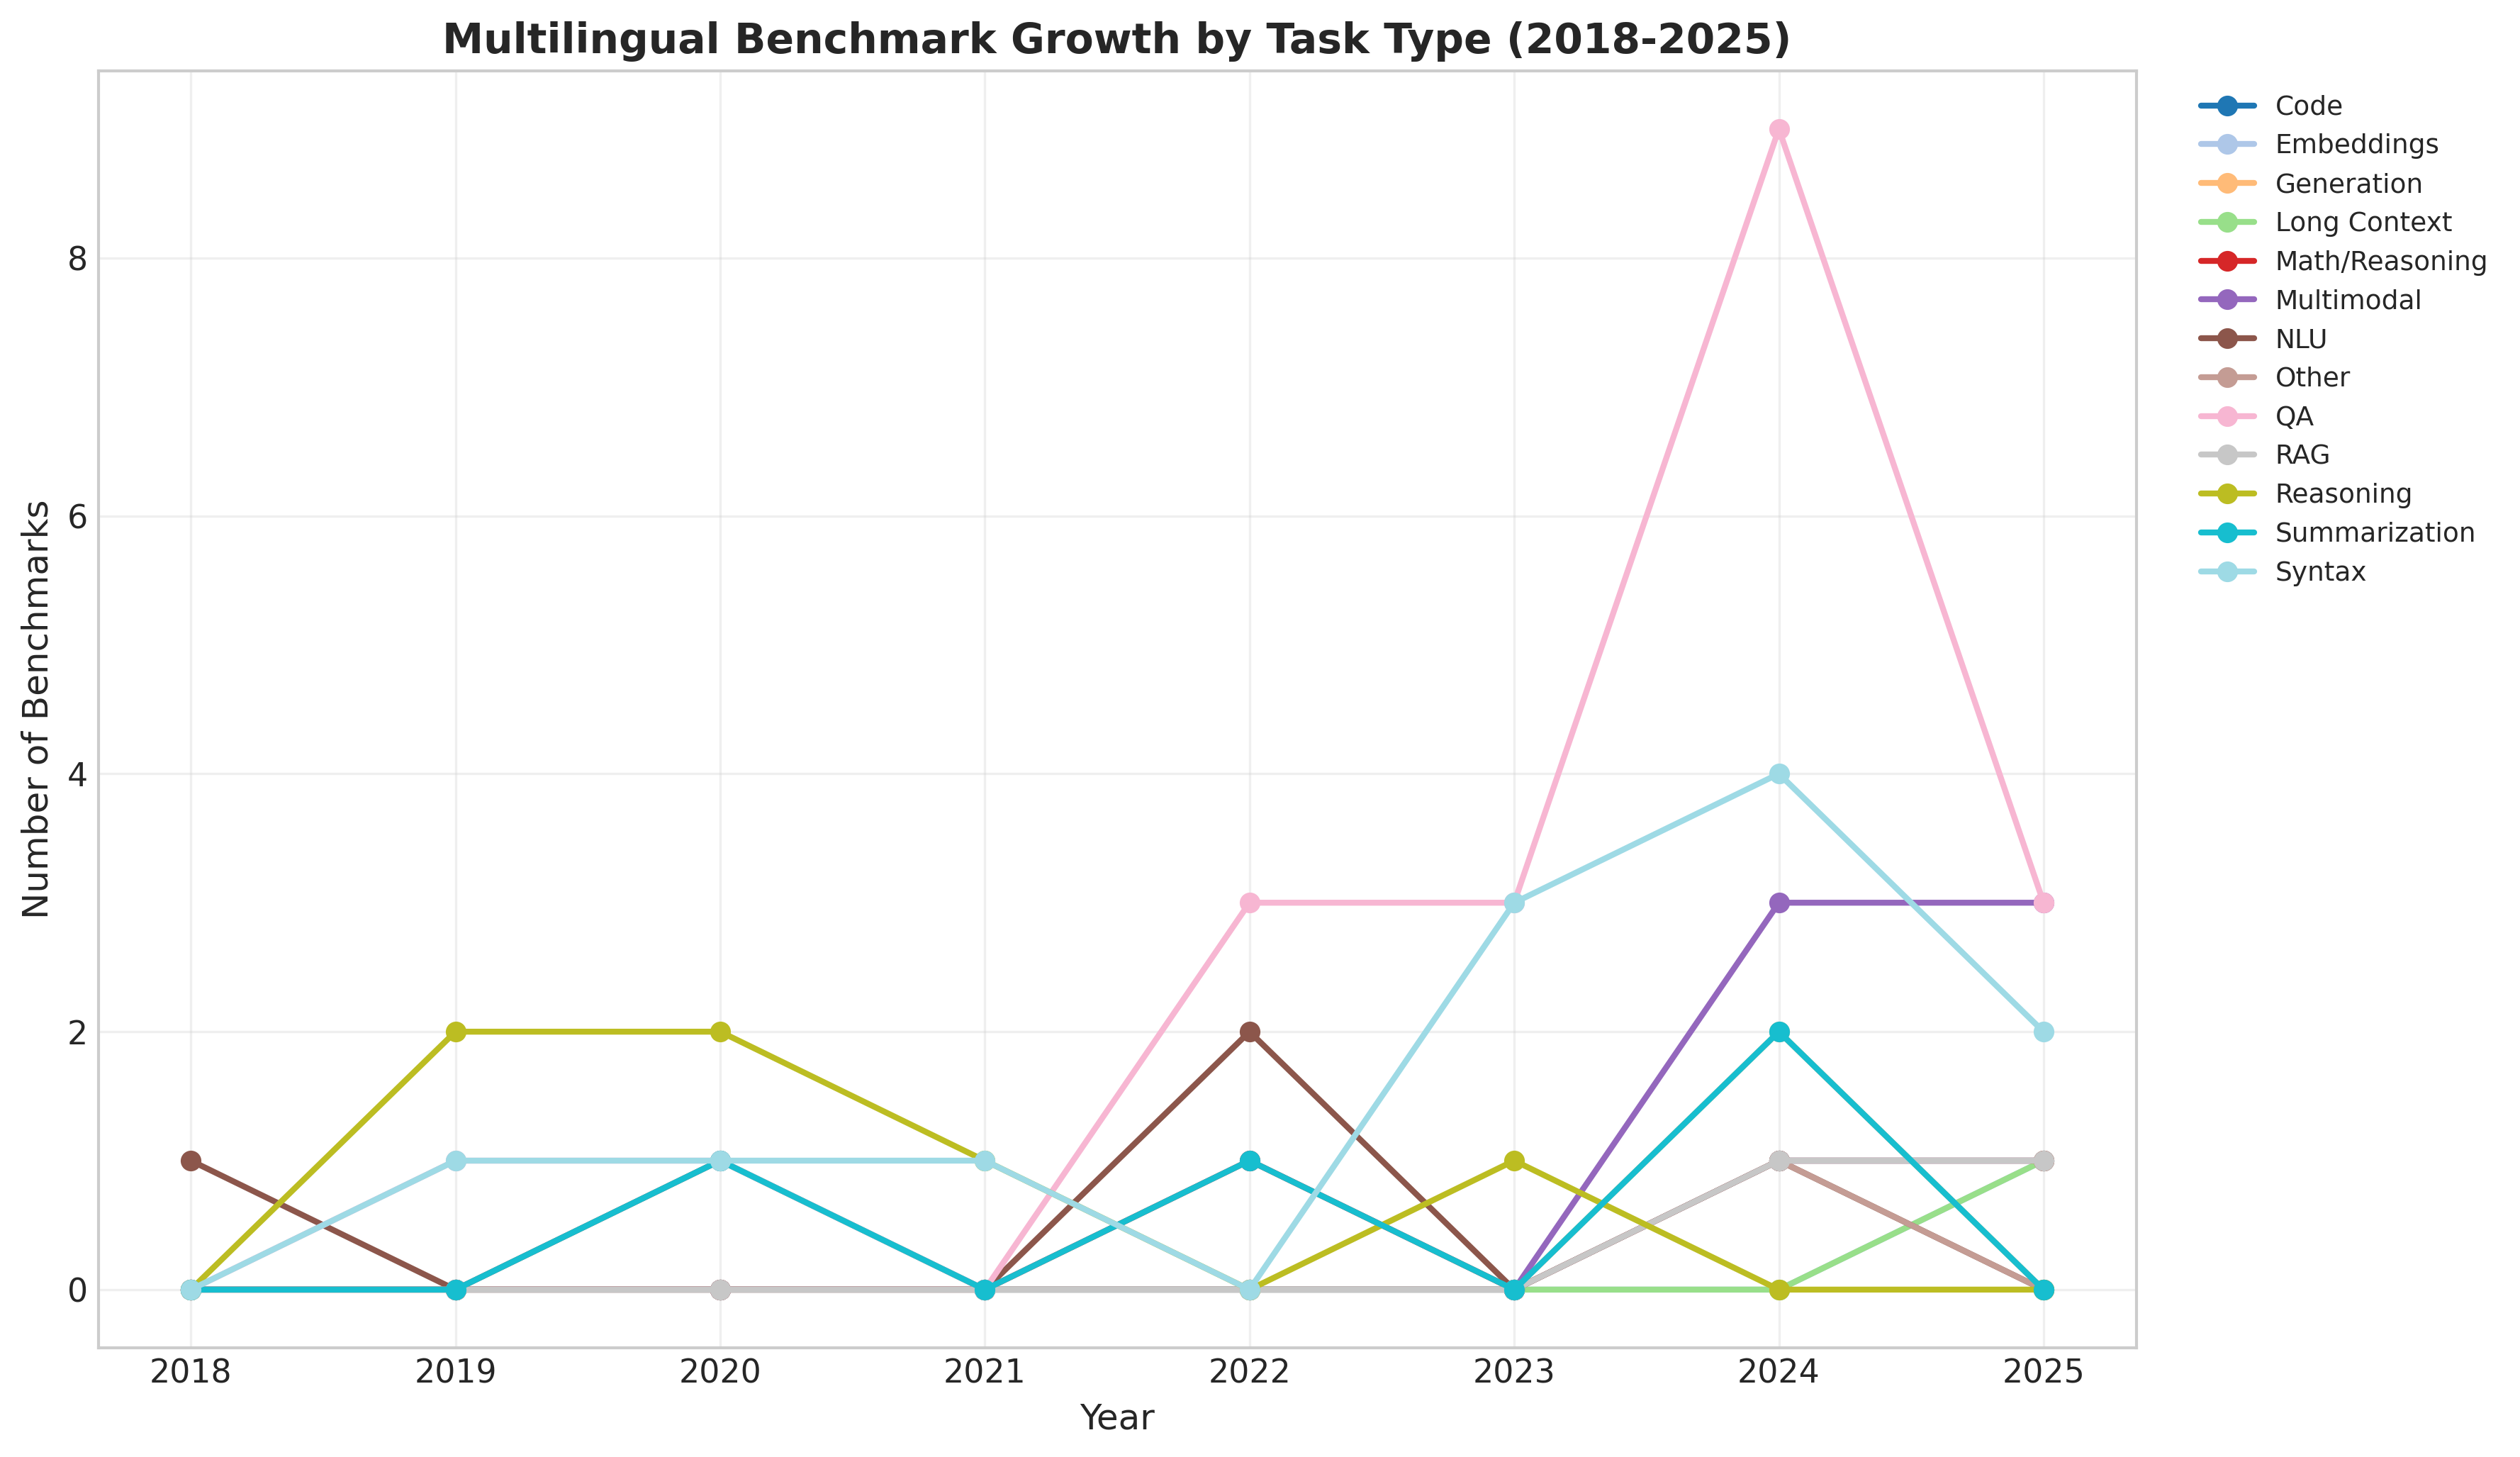
\includegraphics[width=0.8\linewidth]{images/figure2_temporal_complete.png}
    \caption{Temporal growth of multilingual evaluation benchmarks by task type (2018-2025). The sharp increase in 2024 reflects growing community interest in multilingual AI evaluation, particularly in QA and reasoning tasks.}
    \label{fig:3_temporal}
\end{figure*}





 \citep{10.1145/3578553} present KenSwQuAD, a Swahili question-answering dataset containing 1,445 story texts annotated with 7,526 QA pairs, with at least five QA pairs per text. The dataset was created from the Kencorpus Swahili corpus using purposive sampling based on text length and genre, and annotated by trained native speakers following structured guidelines to ensure consistent question types and answer constraints. Quality control on 12.5\% of the dataset (180 texts, 900 QA pairs) showed 53.9\% exact matches, 37.9\% contextually similar answers, 3.8\% minor errors, and 4.4\% disagreement, with third-party review confirming 75\% of disagreements as valid. Proof-of-concept experiments included a semantic network method converting texts into subject-predicate-object triples queried via SPARQL, achieving 80\% Precision@1, and a BERT-based transformer model (XLM-RoBERTa) fine-tuned on the dataset, achieving 59.4\% F1 score and 48\% Exact Match. These results demonstrate moderate performance constrained by limited training data but establish KenSwQuAD as a high-quality benchmark for Swahili QA research, with potential for adaptation to other low-resource languages such as Dholuo and Luhya.

 \citep{heinrich-etal-2022-fquad2} present FQuAD2.0, a French adversarial Question Answering dataset extending FQuAD1.1 with over 17,000 unanswerable questions, totaling nearly 80,000 questions. The dataset enables training QA models that can distinguish unanswerable from answerable questions. CamemBERT models (BASE and LARGE) were fine-tuned on FQuAD2.0, with CamemBERTLARGE achieving 83\% F1 and 82.3\% NoAnsF1. The study shows larger models benefit more from fewer adversarial examples and demonstrates that FQuAD2.0 is more challenging than English SQuAD2.0 under similar conditions. Multilingual experiments with XLM-RoBERTa indicate English-trained models perform reasonably in French zero-shot settings but are outperformed by French monolingual models. The adversarial questions are categorized into antonym negations, entity swaps, ambiguity, out-of-context, and semantic similarity. The authors also discuss model compression techniques (pruning, distillation, quantization) and suggest further dataset expansion, establishing FQuAD2.0 as the first native French adversarial QA benchmark and a key resource bridging French and English QA research.

\subsubsection{QA}
\citep{singh2024global} present Global-MMLU, an improved multilingual benchmark designed to understand and address the significant cultural and linguistic biases in existing evaluation datasets. While the common practice for multilingual assessment is to machine-translate English benchmarks like MMLU, these evaluations often perpetuate a strong Western-centric bias and introduce translation artifacts, distorting model rankings and reducing their utility as true global benchmarks. To address this, the authors release Global-MMLU, an evaluation suite spanning 42 languages with higher-quality translations verified by professional and community annotators. They introduce a novel framework that splits the benchmark into designated Culturally-Sensitive (CS) and Culturally-Agnostic (CA) subsets, allowing for a more holistic evaluation that can distinguish between universal knowledge and culturally-specific understanding. The analysis reveals that 28\% of MMLU questions require culturally sensitive knowledge, with 84.9\% of its geographic questions focused on North America or Europe. Results from re-evaluating 14 models demonstrate that rankings change significantly depending on the subset, with performance on CS data showing far greater variability, highlighting the distortions caused by relying on translated MMLU. The key strength of this work lies in providing the research community with a comprehensive, high-quality, and culturally-aware evaluation suite that offers a more reliable measure of a model's true multilingual capabilities, moving beyond Western-centric evaluation paradigms.

\begin{figure*}[h!]
    \centering
    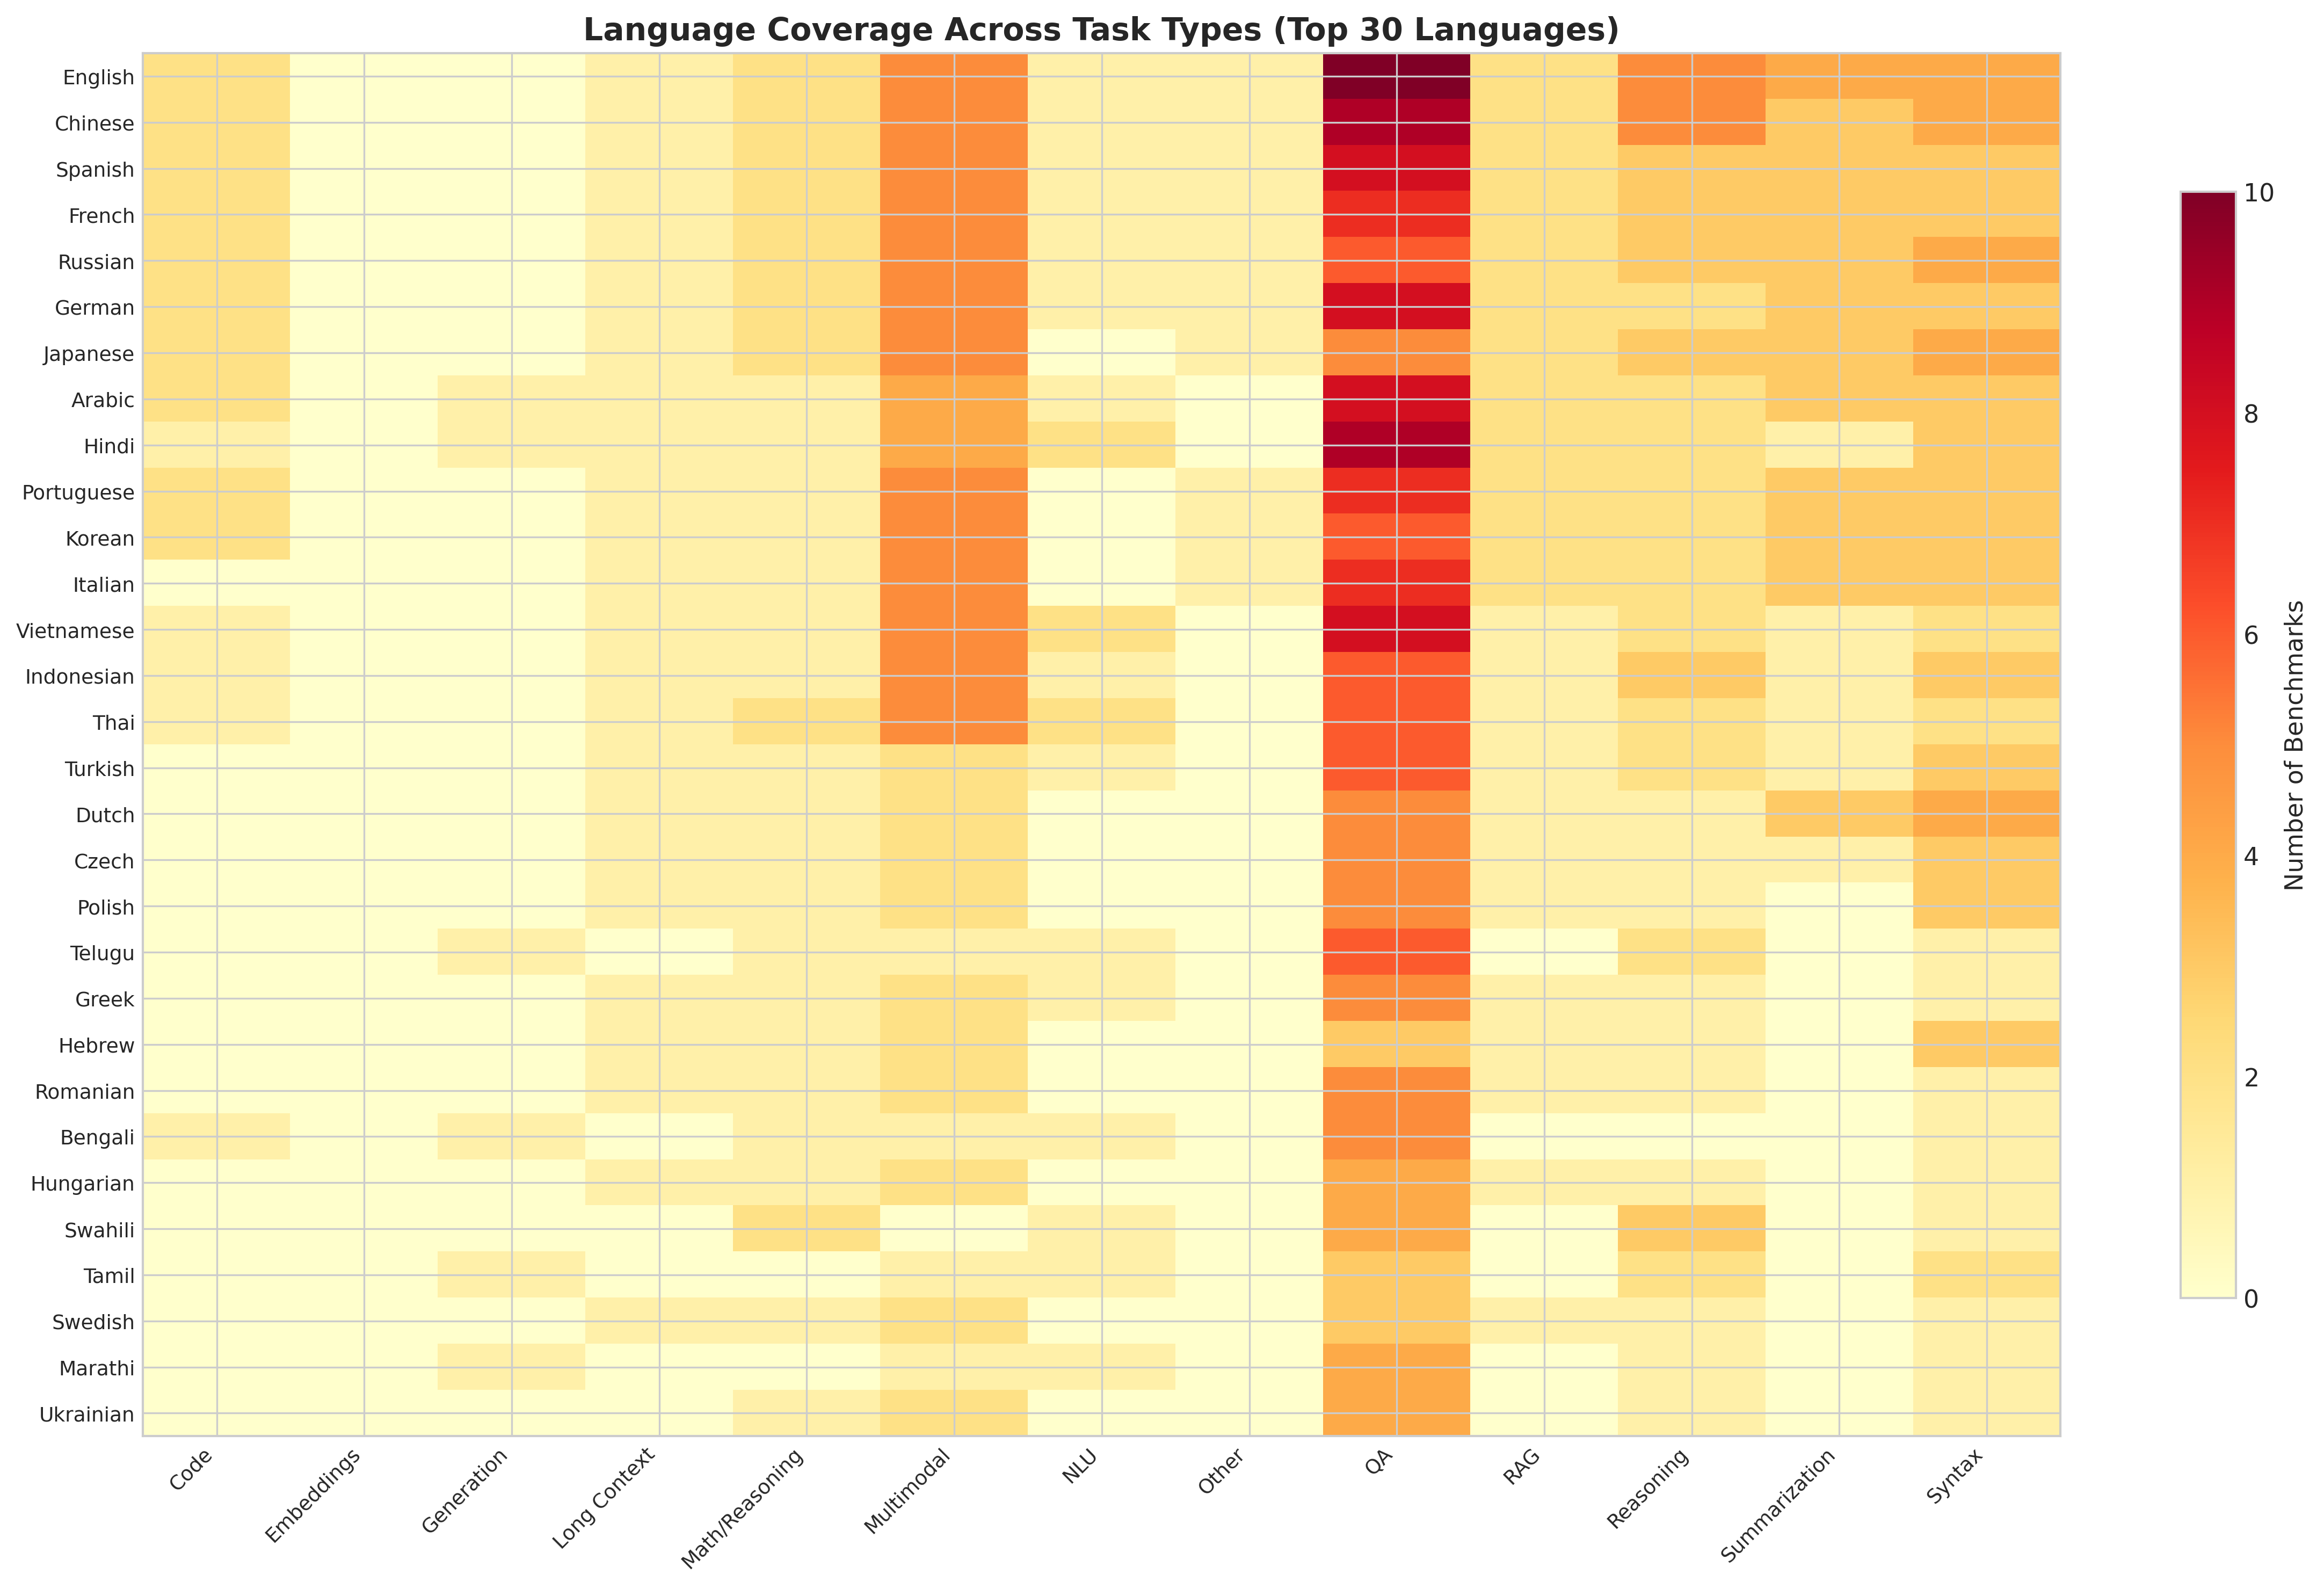
\includegraphics[width=0.8\linewidth]{images/figure3_heatmap_complete.png}
    \caption{Language coverage across task types for the top 30 languages. English, Chinese, Spanish, and French show the highest coverage, while low-resource languages like Swahili, Tamil, and Bengali have limited representation, particularly in specialized tasks.}
    \label{fig:4_heatmap}
\end{figure*}

 \citep{sankalp2025indicmmlu} present IndicMMLU-Pro, a comprehensive benchmark designed to evaluate Large Language Models (LLMs) on massive multitask language understanding across major Indic languages. While Indic languages are spoken by over 1.5 billion people, they have historically been underrepresented in NLP, lacking the rigorous, standardized evaluation frameworks available for dominant languages. To address this gap, the authors created the benchmark by translating the English MMLU-Pro dataset into nine Indic languages—Hindi, Bengali, Gujarati, Marathi, Kannada, Punjabi, Tamil, Telugu, and Urdu—using the IndicTrans2 model. They introduce a robust quality assurance pipeline that includes back-translation, automated evaluation against multiple metrics (chrF++, BLEU, METEOR, TER, and SacreBLEU), and manual proofreading of 9,000 sentence pairs by 13 expert reviewers to ensure semantic accuracy and linguistic style. The benchmark retains the original MMLU-Pro structure and task taxonomy to ensure consistency and facilitate comprehensive evaluation. Baseline results from state-of-the-art models show that GPT-40 consistently outperforms all other models across all nine languages, with accuracy scores ranging from 38.46\% to 44.80\%, establishing a new top performance tier. The key strength of this work lies in providing the community with a publicly available, high-quality, and standardized benchmark that pushes the research boundaries for Indic language AI and enables the development of more accurate and culturally sensitive models.

\citep{xuan2025mmlu} present MMLU-ProX, a comprehensive multilingual benchmark designed to rigorously evaluate the advanced reasoning capabilities of large language models across 29 languages. While LLM evaluation has advanced, existing benchmarks are either limited to a single language or, if multilingual, lack the reasoning difficulty and consistent translation quality needed to assess SOTA models. To address this, the authors extend the challenging MMLU-Pro benchmark, creating 11,829 parallel questions for each of the 29 typologically diverse languages, with a smaller "lite" version of 658 questions for efficient evaluation. They introduce a rigorous semi-automated translation framework that leverages a powerful LLM for initial translation, self-reflection, and improvement, followed by verification from different LLMs and a final comprehensive review by over 30 human experts to ensure high linguistic accuracy and cultural relevance. A systematic evaluation of 36 LLMs reveals significant performance disparities, with models performing well on high-resource languages but showing a marked decline of up to 24.3\% in low-resource languages; reasoning-enhanced models demonstrated better multilingual generalization. The key strength of this work lies in providing the community with a high-difficulty, high-quality, and parallel benchmark that enables the direct comparison of advanced reasoning abilities across diverse languages, setting a new standard for comprehensive multilingual LLM evaluation.

\citep{koto2024arabicmmlu} present ArabicMMLU, the first massive multitask language understanding benchmark designed to evaluate the reasoning and knowledge-intensive capabilities of language models in Arabic. While many state-of-the-art models are trained on Arabic text, their evaluation often relies on datasets translated from English, which introduces biases and fails to assess knowledge specific to the Arabic-speaking world. To address this, the authors constructed a new dataset of 14,575 multiple-choice questions across 40 tasks, sourced directly from school and professional exams in eight countries across North Africa, the Levant, and the Gulf regions. The benchmark was carefully curated in collaboration with native Arabic speakers to ensure rich local context, with over 50\% of questions tailored to Arabic-specific topics like regional history, law, and Islamic studies. A comprehensive evaluation of 35 models revealed substantial room for improvement, with leading open-source models like LLaMA2 and Falcon struggling to perform well, and the top Arabic-centric model, Jais-chat, achieving only 62.3\% accuracy. GPT-4 performed best at 72.5\%, though this was lower than its reported score on translated MMLU, suggesting ArabicMMLU is a more challenging and authentic benchmark. The key strength of this work lies in providing the community with the first large-scale, culturally-localized benchmark for Arabic, enabling a more accurate assessment of LLMs and fostering the development of models with deeper regional understanding.

\citep{li2023cmmlu} present CMMLU, a comprehensive benchmark designed to evaluate the advanced knowledge and reasoning abilities of Large Language Models (LLMs) specifically within a Chinese linguistic and cultural context. While popular benchmarks like MMLU are effective for English, their inherent Western cultural bias makes them unsuitable for accurately assessing model capabilities in other languages. To address this, the authors manually constructed a new dataset of 11,528 multiple-choice questions covering 67 diverse subjects, ranging from STEM and humanities to topics with unique Chinese context, such as driving rules and traditional medicine. The data was carefully collected by human annotators from non-public sources and mock exams to minimize the risk of training data contamination. A thorough evaluation of over 20 LLMs revealed that most models struggle to achieve 60\% accuracy, with GPT-4 leading at 71\%. Notably, the best Chinese-oriented model, Baichuan2-13B, outperformed much larger multilingual models like LLaMA2-70B, highlighting the value of high-quality, language-specific training data. The key strength of this work lies in providing a publicly available, comprehensive, and culturally-grounded benchmark that fills a critical gap in Chinese LLM evaluation and demonstrates that smaller models trained on high-quality monolingual data can be highly competitive for language-specific understanding.

 \citep{yuksel2024turkishmmlu} present TurkishMMLU, the first multitask, multiple-choice question-answering benchmark designed to evaluate the language understanding capabilities of Large Language Models (LLMs) in Turkish. While many multilingual benchmarks rely on automatic translation, this approach can be error-prone and introduce cultural biases. To address this, the authors created a new benchmark of over 10,000 questions covering nine subjects from the Turkish high school curriculum, including culturally specific topics like Turkish Literature and history. The dataset was curated from a high-quality online platform created by the Turkish Ministry of Education, with questions written by curriculum experts, and features a unique "correctness ratio" for each question based on actual student performance to indicate difficulty. A comprehensive evaluation of over 20 LLMs—including open-source, closed-source, and Turkish-adapted models—revealed that closed-source models significantly outperform open-source ones, with GPT-4o achieving the top score of 83.1\%. The best open-source model, Llama-3 70B-IT, scored 67.3\%, highlighting a substantial performance gap. The key strength of this work lies in providing a high-quality, culturally relevant benchmark sourced from expert-created educational materials, which establishes a robust standard for evaluating the Turkish capabilities of LLMs and offers deep insights into their current limitations.

  \citep{son2024kmmlu} present KMMLU, a comprehensive benchmark with 35,030 expert-level multiple-choice questions designed to rigorously evaluate the multitask language understanding of Large Language Models (LLMs) in Korean. While prior Korean evaluation tools have relied on translated versions of English benchmarks, this approach suffers from translation errors and fails to assess knowledge of unique Korean linguistic and cultural nuances. To address this, the authors created a new benchmark sourced entirely from original Korean exams—spanning 45 subjects from humanities to STEM—without any translated material. The benchmark is uniquely tailored to the Korean context, with one-fifth of its questions requiring specific cultural, regional, or legal knowledge for correct resolution. An extensive evaluation of 24 LLMs reveals significant room for improvement, with the top-performing model, GPT-4, scoring just 59.95\%, far below the typical 80\% pass mark on the source exams. Notably, the Korean-specific model HyperCLOVA X outperformed GPT-4 on subjects requiring localized knowledge, such as Korean History. The key strength of this work lies in providing the community with a large-scale, publicly available, and culturally authentic benchmark that captures the specific linguistic aspects of the Korean language, offering a more accurate reflection of model capabilities than translated datasets.

  \citep{yang2019paws} present PAWS-X, a cross-lingual adversarial dataset designed to rigorously evaluate paraphrase identification models across multiple languages. While adversarial datasets like the original PAWS have been effective at exposing model weaknesses, prior work has focused almost exclusively on English, leaving a gap in challenging evaluation data for other languages. To address this, the authors created a new dataset of 23,659 human-translated paraphrase pairs in six typologically distinct languages—French, Spanish, German, Chinese, Japanese, and Korean—by extending the challenging examples from the original PAWS evaluation set. The dataset consists of adversarially constructed pairs with high lexical overlap but potentially different meanings, specifically designed to test a model's sensitivity to sentence structure and context rather than simple word-matching. Evaluations of several models show that Multilingual BERT, when fine-tuned on the English PAWS training data plus machine-translated data for other languages, performs best, achieving an average accuracy gain of 23\% over the next best model across the six non-English languages. The key strength of this work lies in providing the community with a high-quality, human-translated, and challenging multilingual benchmark that effectively measures the cross-lingual capabilities of models and sets a new challenge for developing systems that better capture structure and context.

  \citep{dang2024aya} introduce the Aya Expanse model family, a new generation of 8B and 32B open-weight multilingual language models designed to set a new state-of-the-art in multilingual performance. While LLMs have advanced, a stark performance gap persists across languages, leading to biases, higher costs for underrepresented languages, and safety flaws. To address this, the authors leverage a suite of innovative methodologies including multilingual data arbitrage for synthetic data generation, a multi-stage iterative preference training pipeline, and model merging to maximize diversity and cross-lingual transfer. To facilitate a comprehensive assessment, the authors also introduce m-ArenaHard, a new multilingual evaluation dataset translated from Arena-Hard-Auto into 23 languages. Evaluations show that Aya Expanse models outperform leading open-weight competitors in their respective parameter classes, with the 32B model notably surpassing Llama 3.1 70B—a model with more than twice the parameters—with a 54.0\% win-rate on m-ArenaHard. The key strength of this work lies in successfully combining multiple research breakthroughs into a unified post-training recipe to create highly capable, open-weight multilingual models that significantly close the language performance gap and establish a new frontier for inclusive AI.

\citep{hupkes2025multiloko} present MultiLoKo, a new benchmark designed to evaluate multilinguality in Large Language Models (LLMs) with a focus on locally relevant knowledge across 31 languages. While current multilingual evaluation is insufficient, often relying on translated English benchmarks that introduce cultural biases and translation artifacts, MultiLoKo addresses this by sourcing new, locally-relevant questions for each language. To facilitate a robust analysis, the authors created a main partition of 500 questions per language and also commissioned both human- and machine-authored translations of all non-English questions to and from English, creating parallel datasets. The benchmark is split into a public development set and a blind test set and introduces metrics to assess not only average performance but also performance parity, knowledge transfer, and the impact of using translated versus locally-sourced data. An evaluation of 11 multilingual LLMs reveals that none perform well, with the top model achieving only a 34.4\% average score and showing large performance gaps across languages. A significant "mother tongue effect" was also observed, indicating suboptimal knowledge transfer between languages. The key strength of this work lies in providing a wide-coverage, locally-sourced benchmark that moves beyond the English-centric bias of translated datasets, enabling not only a more authentic evaluation of LLMs but also a meta-analysis of how benchmark design choices impact evaluation outcomes.

\citep{huang2025benchmaxcomprehensivemultilingualevaluation} introduce BenchMAX, a comprehensive multilingual evaluation suite covering 17 languages from 11 families and designed to assess six advanced capabilities of LLMs: instruction following, reasoning (math/science), code generation, long-context understanding, tool use, and translation. Data is machine-translated from English and post-edited by three native annotators, with GPT-4o-mini used as an LLM-judge to finalize translations, ensuring high quality. BenchMAX includes challenging tasks such as HumanEval+ for code completion, LiveCodeBench for problem solving, MGSM for math reasoning, GPQA for science reasoning, RULER for long-context QA, and Nexus for multilingual tool use. Experiments with LLaMA-3.1, Qwen2.5, Gemma2, Aya-Expanse, InternLM2.5, DeepSeek-V3, and GPT-4o-mini show that while larger models improve average performance, gaps between English and non-English remain, especially for low-resource languages (e.g., Telugu, Swahili, Bengali), and domain-specific translation proves particularly challenging. The study highlights that model scaling alone cannot close multilingual disparities, positioning BenchMAX as a high-quality benchmark for probing language-agnostic yet uneven multilingual capabilities in state-of-the-art LLMs.

\citep{zhang2025pmmevalparallelmultilingualmultitask} propose P-MMEval, a parallel multilingual multitask benchmark designed to consistently evaluate LLMs across both fundamental NLP and capability-specialized tasks. It unifies eight benchmarks spanning XNLI, MHELLASWAG, FLORES-200 (translation), MGSM (math reasoning), MMMLU (knowledge), MLOGIQA (logical reasoning), HUMANEVAL-XL (code generation), and MIFEVAL (instruction following), covering 10 languages from 7 families with expert-reviewed translations to ensure fidelity and parallelism. Evaluation of open- and closed-source models (Qwen2.5, LLaMA-3, Gemma2, Mistral, GPT-4o, Claude-3.7) shows that larger models consistently improve multilingual transfer, though with strong task and language variation: code and math transfer best, logical reasoning transfers worst, and Thai/Japanese lag behind Spanish/Portuguese due to data/resource imbalance. To quantify transfer, the authors introduce the Cross-lingual Accuracy Consistency Ratio (CACR), showing that benchmark origin (English vs. Chinese) strongly impacts measured transfer success. Overall, P-MMEval provides the most comprehensive and parallel evaluation suite to date, enabling systematic study of multilingual performance and cross-lingual transfer.

\begin{table}[htbp]
\centering
\caption{Benchmark-Dataset Comparison by Task Class}
\label{tab:benchmark-dataset-comparison}
\begin{tabular}{lccc}
\toprule
\textbf{Task Class} & \textbf{Dataset Count} & \textbf{Benchmark Count} & \textbf{Ratio} \\
\midrule
QA & 4 & 20 & 1:5 \\
Syntax & 20 & 12 & 1.7:1 \\
NLU & 15 & 5 & 3:1 \\
Reasoning & 2 & 6 & 1:3 \\
Translation/MT & 8 & -- & -- \\
Multimodal & 1 & 6 & 1:6 \\
Code & 3 & 2 & 1.5:1 \\
Summarization & 20 & 4 & 5:1 \\
\bottomrule
\end{tabular}
\end{table}

\subsubsection{Syntax}
\noindent

\citep{jumelet2025multiblimp10massivelymultilingual} present MultiBLiMP 1.0, a large-scale multilingual benchmark of linguistic minimal pairs designed to evaluate large language models’ (LLMs) formal syntactic competence across 101 languages and over 128,000 minimal pairs. The dataset focuses on subject-verb and subject-participle agreement for number, person, and gender, and is generated via an automated pipeline leveraging Universal Dependencies and UniMorph, which extracts candidate structures, validates agreement statistically, inflects words to create ungrammatical counterparts, and balances lexical diversity. MultiBLiMP extends prior monolingual and limited multilingual syntactic evaluation efforts by explicitly disentangling formal syntactic competence from functional or semantic evaluation. Evaluations of 42 LLMs, including multilingual models such as Llama3, Gemma3, and Qwen3, reveal that linguistic competence correlates strongly with model size and language frequency in training data, while post-training (instruction tuning) can reduce multilingual fluency. Notably, monolingual models trained on sufficient data outperform larger multilingual LLMs on several languages. The benchmark underscores the continued importance of linguistic resources like UD and UniMorph, offers insights into multilingual model training strategies, and enables future research in computational typology and broader syntactic phenomena.

\citep{warstadt2023blimpbenchmarklinguisticminimal} present BLiMP, a large-scale linguistically motivated benchmark designed to evaluate the grammatical knowledge of language models (LMs) across 67 paradigms covering 12 major English grammatical phenomena, including agreement, binding, control/raising, ellipsis, filler-gap dependencies, irregular forms, island effects, negative polarity item licensing, argument structure, quantifiers, and subject-verb agreement. The dataset is generated using linguist-crafted grammar templates to create controlled minimal pairs contrasting acceptability, validated with human judgments showing 96.4\% agreement. BLiMP evaluates model architectures including n-gram, LSTM, Transformer-XL, and GPT-2, by comparing their probabilities for grammatical versus ungrammatical sentences without supervision. Results show that state-of-the-art models perform well on morphological agreement and some syntactic phenomena but struggle with semantic phenomena such as NPI licensing, argument structure, and syntactic islands, underperforming humans. The study also finds that training data volume impacts linguistic knowledge acquisition more than model size and confirms that full-sentence and prefix-based evaluation methods yield consistent assessments. BLiMP complements benchmarks like CoLA and GLUE, providing a fine-grained, unsupervised tool for assessing grammatical sensitivity and guiding improvements in neural language modeling.

\citep{liu2024zhoblimpsystematicassessmentlanguage} present ZhoBLiMP, a comprehensive Chinese linguistic minimal pairs benchmark consisting of 35,000 minimal pairs across 118 paradigms covering 15 linguistic phenomena. The dataset is generated using linguist-crafted grammar templates combined with a curated vocabulary and an intuitive GUI for minimal pair creation. The study evaluates 20 transformer-based models trained from scratch on Chinese corpora ranging from 10M to 3B tokens and 14 off-the-shelf large language models across four families, using mean log-probability metrics. Results indicate that models with ~410M parameters trained on 1B tokens for one epoch can learn much of Chinese grammar, though phenomena like anaphor resolution, ellipsis, and quantifiers remain challenging, highlighting the need for discourse-level knowledge. U-shaped learning curves were observed, mirroring child language acquisition patterns, with phrase-level knowledge preceding sentence-level long-distance dependencies. This work fills a gap in non-English syntactic evaluation, providing a robust tool for probing Chinese linguistic competence and enabling comparative studies across languages.

\citep{başar2025turblimpturkishbenchmarklinguistic} present TurBLiMP, the first comprehensive Turkish linguistic minimal pairs benchmark, covering 16 grammatical phenomena including flexible word order and morphological subordination. The dataset contains 16,000 minimal pairs (1,000 per phenomenon) plus 2,000 additional pairs testing experimental paradigms on word order and subordination, created through manual crafting, semi-automatic augmentation using BERTurk, and fully automated lexical replacements. Human acceptability judgments from 30 native speakers using a 7-point Likert scale validated the dataset, revealing varied model-human alignment across phenomena. Thirteen monolingual and multilingual models, including BERTurk, cosmosGPT, EuroLLM, Gemma, and Qwen, were evaluated using sequence log probabilities, showing that larger models generally perform better, but monolingual Turkish models often surpass larger multilingual ones. Results highlight challenges in ellipsis, island effects, and relative clauses, with experimental paradigms revealing model sensitivity to non-canonical word orders and subordination types. BERTurk correlated best with human judgments, demonstrating masked LM advantages. TurBLiMP provides a linguistically motivated, high-quality benchmark that advances evaluation of Turkish LMs beyond BLiMP and MultiBLiMP, addressing typological gaps in agglutinative and free word order languages while supporting language-specific model development and nuanced syntactic competence analysis.

\citep{frank_suijkerbuijk_prins_de_heer_kloots_zuidema_2025} introduce BLiMP-NL, a comprehensive Dutch minimal pair corpus designed for benchmarking language models, inspired by the English BLiMP dataset but improving methodology through hand-crafted and native speaker-validated sentence pairs. The dataset spans 84 paradigms across 22 syntactic phenomena, controlling for confounds such as word frequency in critical regions, and incorporates graded human acceptability ratings and reading times beyond typical binary judgments. Large-scale generation leverages GPT-3.5 Turbo, with manual validation ensuring naturalness and targeted grammatical contrast. BLiMP-NL evaluates a wide range of Dutch and multilingual LMs—including encoders (BERTje, RoBERTa, XLM-RoBERTa) and decoders (GPT-2, Llama, Mistral/GEITje)—using intrinsic (probability-based, SLOR) and extrinsic (prompting) metrics, revealing that models differ across linguistic phenomena, larger model size does not guarantee better grammar performance, and prompting is less reliable than probability-based evaluation. The dataset provides robust recommendations for dataset design, evaluation practices, and cross-linguistic research, establishing a key resource for probing grammar sensitivity and human-likeness in Dutch language models.

\citep{taktasheva-etal-2024-rublimp} present RuBLiMP, the first large-scale, multidomain benchmark of 45,000 Russian linguistic minimal pairs spanning 45 paradigms across 12 morphological, syntactic, and semantic phenomena. The dataset is constructed from open corpora (Wikipedia, Wikinews, Librusec), annotated with a state-of-the-art multidomain morphosyntactic parser, and transformed into minimal pairs via expert-written perturbation rules targeting morphological inflection, syntactic agreement, government, negation, argument structure, aspect, and tense. To prevent contamination from LM pretraining data, a MIN-K\% PROB filtering step is applied. Human validation by 20 linguistically trained native speakers confirmed high quality and inter-annotator agreement. Evaluations of 25 monolingual and multilingual Transformer-based models revealed strong sensitivity to morphological and agreement contrasts but challenges with structural relations, negation, transitivity, and tense, with monolingual models generally outperforming multilingual ones and larger models not always performing better. RuBLiMP’s scale, domain diversity, and high-quality verification distinguish it from existing benchmarks like BLiMP, CLiMP, JBLiMP, SLING, NoCoLAzero, DaLAJ, LINDSEA, and CLAMS, providing a robust resource for Russian linguistic evaluation and advancing methodologies in minimal pair generation, pretraining data filtering, and empirical model analysis.

\citep{someya-oseki-2023-jblimp}  present JBLiMP, a Japanese Benchmark of Linguistic Minimal Pairs, a dataset for targeted syntactic evaluation of language models in Japanese. JBLiMP comprises 331 minimal pairs covering 11 linguistic phenomena, including argument structure, binding, verbal agreement, and filler-gap dependencies, derived from acceptability judgments in Japanese theoretical linguistics journal articles (JEAL). The dataset combines complex phenomena coverage, akin to CoLA, with minimal pair sentence presentation, as in BLiMP. Evaluation of GPT-2, LSTM, and n-gram models trained on a large Japanese corpus using SLOR scores showed overall syntactic accuracy of \textasciitilde75\%, substantially below the human baseline of \textasciitilde91\%. Analysis revealed that models capture local dependencies effectively but struggle with long-distance phenomena such as verbal agreement and binding. JBLiMP provides a linguistically motivated benchmark for probing Japanese syntactic knowledge and highlights the need for comparable datasets in other non-English languages. 


\citep{volodina-etal-2021-dalaj} present DaLAJ 1.0, a Swedish linguistic acceptability dataset derived from the SweLL learner corpus, comprising 9,596 sentences each containing a single lexical error spanning four types relevant for semantic interpretation (L-W, L-Der, L-FL, O-Comp). Unlike artificially generated datasets such as CoLA, DaLAJ leverages authentic learner errors with expert-annotated corrections and metadata on mother tongue and proficiency. Sentences are organized as correct/incorrect pairs focusing on one error per sentence, facilitating model training and evaluation for acceptability classification and aligning with SwedishGlue for broader Swedish NLU benchmarking. The study addresses ethical and legal challenges related to learner data under GDPR, using sentence scrambling and restricted metadata to enable wider access. Initial baselines for binary acceptability classification are established, with plans to extend to error detection, classification, and correction, positioning DaLAJ as a key resource for Swedish NLP research and language learning applications.

\citep{leong2023bhasaholisticsoutheastasian} introduced **LINDSEA**, a high-quality diagnostic dataset for Indonesian and Tamil designed to evaluate LLMs’ linguistic abilities across syntax, semantics, and pragmatics. It complements the BHASA NLP benchmark with four test formats: minimal pairs, translation, information recovery, and binary choice, validated by multiple native speakers (inter-annotator agreement 94.89–100\%). GPT-4 outperformed GPT-3.5-Turbo overall, especially in Indonesian (syntax 64.7\%, semantics 66.4\%, pragmatics 70.8\%, overall 67.3\%) versus Tamil (syntax 52.1\%, semantics 59.3\%, pragmatics 48.3\%, overall 48.3\%), but gaps remain. GPT-4 handled Indonesian NPIs, negation, relative clauses, and word order well, but struggled with voice affixes, enclitics, and reflexives; in Tamil, it struggled with case markers, subject-verb agreement, scrambling, complementizers, and complex predicates. Translation and coreference tasks were easier in Indonesian (GPT-4 69.7\% and 74.5\%) than Tamil (43.8\% and 24.4\%), with idiomatic expressions and verbal reduplication being particularly challenging. Pragmatic reasoning was slightly better, but overall results show both models fall short of native-like proficiency.


\citep{gauthier2020syntaxgym}- This paper presents SyntaxGym, a platform built to evaluate whether neural language models genuinely capture human-like syntactic generalizations. Rather than relying on broad measures like perplexity, it uses targeted, psycholinguistically inspired tests such as subject–verb agreement in controlled sentence pairs. The authors introduce both a web interface and two supporting command-line tools: syntaxgym, which automates the evaluation process, and lm-zoo, which standardizes model interaction using Docker APIs. This dual setup makes the framework accessible to linguists who want to design experiments without coding overhead, while also enabling NLP researchers to easily submit and test their models. A key strength is its focus on reproducibility and fine-grained evaluation, looking at specific sentence regions instead of just whole-sentence probabilities, setting it apart from resources like BLiMP. The platform is seeded with 33 test suites and 8 state-of-the-art models, providing an immediate, community-driven resource that bridges linguistic theory with modern NLP practice.

\citep{unknown} benchmark extends the COMPS dataset into a multilingual conceptual minimal pair suite spanning 17 languages across analytic, inflectional, and agglutinative typologies. It probes LLMs’ ability to associate concepts with properties (e.g., toaster → used for heating food) independent of language, using four types of negative samples: taxonomic, property-overlap, co-occurrence, and random. To evaluate both performance and competence, the authors adopt a three-pronged framework: (i) metalinguistic prompting (explicit task performance), (ii) direct probability measurement (implicit preferences), and (iii) neurolinguistic probing (internal conceptual representations). Experiments on LLaMA 3.1 (base, instruction-tuned, and knowledge-distilled) reveal that: (1) LLMs’ conceptual reasoning degrades in low-resource and morphologically complex languages, with cross-linguistic generalization far from universal; (2) models succeed on distinct contrasts but falter on subtle semantic distinctions; (3) instruction tuning boosts performance without improving internal competence, whereas knowledge distillation enhances competence for low-resource languages but trades off some performance in high-resource settings; and (4) conceptual knowledge tends to peak at mid-layers, requiring deeper layers for agglutinative languages. Overall, XCOMPS provides the first multilingual conceptual reasoning benchmark, exposing limitations in the universality of LLMs’ semantic reasoning


\subsubsection{Reasoning}
\noindent

\citep{ponti-etal-2020-xcopa} present XCOPA, the first large-scale multilingual dataset for causal commonsense reasoning across 11 typologically diverse languages. The dataset is created by translating and re-annotating English COPA examples to preserve causal relations while ensuring cultural and linguistic naturalness. State-of-the-art multilingual encoders such as XLM-R, mBERT, and multilingual USE are benchmarked under various transfer setups, revealing a “curse of multilinguality” where multilingual models underperform compared to monolingual ones, though XLM-R consistently achieves the best results, especially when pretrained on SIQA. The authors also propose resource-lean adaptation methods for low-resource languages using small monolingual corpora or bilingual dictionaries, yielding substantial improvements over random baselines. XCOPA’s typological, genealogical, and geographical diversity makes it a robust benchmark for evaluating cross-lingual commonsense reasoning.

\citep{cheng2024mubenchmultitaskmultimodalbenchmark} present MU-Bench, the first comprehensive benchmark for machine unlearning (MU) that unifies deleted sample sets, trained models, and evaluation metrics across diverse tasks and modalities, including previously underexplored domains like speech and video. The benchmark evaluates key MU methods such as RANDLABEL, SALUN, BAD-T, SCRUB, and NEGGRAD across 20 architectures and 9 datasets, standardizing deletion ratios and introducing a unified teacher-student taxonomy for measuring knowledge deletion, corruption, and retention. Findings show that RANDLABEL and SALUN are the most robust methods with higher deletion capacity, while BAD-T can reach near-random performance on deletion sets but with smaller capacity and higher computational cost; SCRUB shows mixed success, and NEGGRAD underperforms in most cases. MU-Bench also highlights challenges in audio, video, and generative tasks and explores factors like parameter-efficient fine-tuning, curriculum learning, MU scaling, and bias amplification. The open-source package and leaderboard enable standardized, scalable evaluation, establishing MU-Bench as a foundational platform for fair comparison and advancement in machine unlearning research.

\citep{sakaguchi2019winograndeadversarialwinogradschema} present Winogrande (2019), a large-scale Winograd Schema Challenge (WSC)-inspired dataset comprising 44,000 problems designed to improve both scale and difficulty while reducing dataset-specific biases through a novel adversarial filtering algorithm, AFLITE. The dataset was crowdsourced using creativity-driven constraints and carefully validated to ensure human-level ease, achieving 94.0\% human accuracy, while state-of-the-art models such as RoBERTa reach only 59.4–79.1\%, revealing a substantial performance gap. AFLITE mitigates spurious correlations by iteratively filtering biased instances using RoBERTa embeddings with a logistic regression ensemble, outperforming simpler bias reduction methods. Fine-tuning on Winogrande notably enhances transfer learning, establishing new state-of-the-art results on five related benchmarks: WSC (90.1\%), DPR (93.1\%), COPA (90.6\%), KnowRef (85.6\%), and Winogender (97.1\%). The work underscores concerns about overestimating machine commonsense reasoning due to dataset biases and advocates for algorithmic bias reduction to maintain the reliability of current and future challenge benchmarks. 

 \citep{wang2024seaevalmultilingualfoundationmodels} propose SeaEval, a multilingual benchmark that goes beyond standard NLP tasks to evaluate complex reasoning, cultural understanding, and cross-lingual knowledge transfer across 29 datasets, including 7 newly constructed ones. The benchmark introduces datasets such as SG-Eval, US-Eval, CN-Eval, PH-Eval for cultural reasoning and Cross-MMLU, Cross-LogiQA for consistency testing across 7 languages. Evaluation protocols incorporate not only accuracy but also instruction sensitivity (robustness to paraphrasing) and cross-lingual consistency (AC3 score). Experiments with models including GPT-4, ChatGPT, LLaMA-2, Baichuan-2, and BLOOMZ reveal key limitations: (1) sensitivity to paraphrased prompts, (2) label-order exposure bias, (3) inconsistent answers to semantically equivalent multilingual queries, and (4) persistent imbalance between high- and low-resource languages. While GPT-4 leads in overall accuracy, BLOOMZ shows stronger cross-lingual consistency, though absolute scores remain unsatisfactory, highlighting the difficulty of balanced multilingual contextualization. SeaEval establishes a comprehensive framework for probing linguistic, reasoning, and cultural dimensions of multilingual foundation models.

 
\subsubsection{Multimodal}
\noindent

\citep{zhang2023m3exam} present M3Exam, a multilingual, multimodal, and multilevel benchmark designed to comprehensively evaluate the capabilities of large language and vision-language models. Existing benchmarks for evaluating foundation models often lack diversity, focusing narrowly on a single language (like English), a single modality (like text), or a single educational level. To address this, the authors constructed a new dataset by collecting questions from national college entrance examinations in nine different languages and across a variety of subjects, including both science and humanity disciplines. The key feature of M3Exam is its multifaceted nature, as it contains questions in nine languages, covers three educational levels (primary, secondary, and college entrance), and is the first to include a significant number of multimodal questions that require understanding both text and images to answer correctly. An extensive evaluation of 16 open-source models and 4 proprietary models, including GPT-4, reveals that while models like GPT-4 show strong performance, there is a substantial gap between their capabilities and human performance, particularly in the multimodal and low-resource language settings. The key strength of this work lies in providing a high-quality, human-centric benchmark that captures real-world educational challenges and offers a more holistic and challenging evaluation of foundation models across linguistic, modal, and educational diversities.

\citep{vayani2025languagesmatterevaluatinglmms} ALM-bench is the largest multilingual multimodal evaluation suite to date, spanning 100 languages, 24 scripts, 15 language families, and 73 countries. It provides 22.7K manually verified question-answer pairs across 19 domains, including both generic vision tasks (e.g., indoor/outdoor scenes, food, sketches) and 13 culture-specific categories such as heritage, festivals, customs, notable figures, and religion. ALM-bench introduces four question types (MCQ, True/False, short VQA, long VQA), enabling a comprehensive assessment of linguistic and cultural reasoning. Compared to prior benchmarks like CVQA or MaRVL, ALM-bench covers 3× more languages, broader domain diversity, and richer cultural depth, with over 800 hours of expert native-speaker validation ensuring cultural fidelity. Benchmarking 16 state-of-the-art LMMs shows that while closed-source models (e.g., GPT-4o, Gemini-1.5-Pro) outperform open-source counterparts, all models struggle significantly on low-resource languages and culturally nuanced tasks. For example, GPT-4o achieves 78.8\% overall but drops to ~50\% on Amharic. Error analyses reveal challenges in script handling, cultural grounding, and reasoning, underscoring limitations of current models in truly global multimodal contexts. By releasing this benchmark, the authors establish a culturally and linguistically inclusive standard for evaluating future LMMs

\citep{lovenia2025seacrowdmultilingualmultimodaldata} present the SEACrowd initiative, which advances AI for Southeast Asian (SEA) languages by addressing resource scarcity and the lack of evaluation benchmarks for nearly 1,000 languages across text, vision, and speech. SEACrowd consolidates around 500 standardized datasets with detailed metadata and dataloaders, enabling more accessible and consistent use. Its benchmark suite evaluates 36 indigenous SEA languages on 13 tasks, including natural language understanding (NLU), natural language generation (NLG), automatic speech recognition (ASR), and vision-language (VL) tasks, using both commercial and open-source large language models (LLMs), multilingual vision-language models (VLMs), and speech models. Models such as AYA-101 and mT0 perform strongly in zero-shot settings, while SEA-specific models like SEA-LION and SeaLLM also achieve competitive results, highlighting the importance of regional focus. Speech models like Whisper v3 perform well on major national languages but less effectively on indigenous ones, whereas Seamless M4T v2 shows more balanced performance. Current VLMs still struggle to generate high-quality SEA language image captions, indicating a gap in multilingual vision-language pretraining. Analysis of language generation quality reveals widespread “translationese,” with SEA-LION producing the most natural outputs (\textasciitilde 58\%). Resource distribution remains long-tailed, with most SEA languages underrepresented and cultural grounding limited due to reliance on translated rather than native texts. To address these gaps, SEACrowd proposes prioritization strategies based on potential utility and resource equity, emphasizing investment in both high-resource national languages and severely under-resourced local languages to preserve linguistic diversity and cultural heritage. The initiative also establishes contribution workflows, data standards, and evaluation protocols to sustain and expand SEA AI research and development.

\citep{lovenia2024seacrowd} present SEACrowd, a collaborative, multilingual, and multimodal initiative designed to create a comprehensive data hub and benchmark suite for the underrepresented languages of Southeast Asia (SEA). While SEA is home to over 1,300 languages, the performance of AI models in this region is compromised by a significant lack of datasets and the cultural bias inherent in Anglocentric training data. To address this, the authors launched a collaborative effort to consolidate and standardize approximately 500 corpora for nearly 1,000 SEA languages across text, image, and audio modalities. The initiative introduces the SEACrowd Benchmarks, which facilitate standardized evaluation of AI models across 38 indigenous SEA languages and 13 tasks. An extensive evaluation reveals that models trained on a greater number of SEA languages generally exhibit better performance and higher language equity. Furthermore, the study finds that the generative outputs of current LLMs in SEA languages often resemble "translationese" rather than natural language, with even the best-performing models struggling to produce authentic text. The key strength of this work lies in its massive, collaborative effort to create a centralized and standardized resource hub that bridges a critical resource and evaluation gap, providing crucial insights into the current AI landscape for SEA and paving the way for more equitable and culturally relevant AI development.


\subsubsection{Natural Lanugage Understanding (NLU)}
\noindent

\citep{conneau2018xnlievaluatingcrosslingualsentence} present XNLI (Cross-lingual Natural Language Inference), a large-scale multilingual corpus extending MultiNLI with 7,500 English premise–hypothesis pairs professionally translated into 15 languages, including low-resource ones such as Swahili and Urdu. Each premise is paired with three hypotheses (entailment, contradiction, neutral), validated by multiple annotators to ensure quality. To benchmark cross-lingual learning, the authors evaluate translation-based methods (TRANSLATE TRAIN and TRANSLATE TEST, with the latter generally performing better) alongside multilingual sentence encoders such as X-CBOW (a universal multilingual embedding model) and X-BiLSTM (trained with alignment loss for zero-shot transfer). Results show that translation-based methods yield the highest accuracy, while multilingual encoders provide an efficient alternative that avoids translation at inference time, with max-pooling BiLSTMs achieving up to 73.7\% in English and 58–68\% across other languages. The work underscores the challenges of building annotated multilingual data and highlights the potential of alignment-based embedding techniques, establishing XNLI as a standardized benchmark for multilingual NLP, low-resource language understanding, and cross-lingual transfer learning. 

\cite{aggarwal2022indicxnlievaluatingmultilingualinference} present IndicXNLI, a large-scale Natural Language Inference (NLI) benchmark for eleven major Indic languages, Assamese, Gujarati, Kannada, Malayalam, Marathi, Odia, Punjabi, Tamil, Telugu, Hindi, and Bengali respectively, created by translating the English XNLI dataset (392,702 train, 2,490 validation, 5,010 test examples per language) using the IndicTrans seq2seq model, with quality validated through human annotations (average >0.85) and automatic BERTScore metrics (Pearson >0.7, Spearman >0.8). The dataset supports evaluation of multilingual pre-trained models, including Indic-specific architectures (MuRIL, IndicBERT) and general-purpose ones (mBERT, XLM-RoBERTa), across training strategies such as Indic Train, English Train (zero-shot), Translate-Test (English Eval), English + Indic Train (sequential fine-tuning), Train All (multi-language sequential training), Cross-Lingual Transfer (training on one Indic language, testing on others), and Intra-Bilingual Inference (mixed English–Indic inputs). Results show MuRIL consistently outperforms other models, achieving LangAvg scores of \textasciitilde72–75 across languages, due to its Indic-specific pretraining that combines MLM, TLM, and transliteration. The English + Indic Train strategy yields the strongest performance overall, while cross-lingual transfer works best when training on high-resource languages such as Hindi and Bengali. However, mixed-language inference remains challenging, with generic models like XLM-RoBERTa outperforming Indic-specific ones, underscoring the complexity of bilingual reasoning. By introducing a high-quality benchmark and comprehensive evaluation, IndicXNLI advances multilingual NLP for Indic languages, addressing the resource scarcity in this linguistically diverse region and laying groundwork for integration into IndicGLUE. 


\citep{Amirkhani_2023} present FarsTail, the first large-scale Persian natural language inference (NLI) dataset, comprising 10,367 samples derived from 3,539 multiple-choice questions with minimal annotator intervention, designed to reflect real-world applications similar to SciTail. The dataset uses a multi-step generation and relabeling process to ensure high-quality annotations and is split into balanced train, validation, and test sets. The authors evaluate a wide range of embedding and classification methods, including word embeddings (word2vec, fastText, ELMo, LASER), RNN-based models (LSTM, BiGRU), NLI-specific architectures (DecompAtt, ESIM, HBMP), language model fine-tuning (ULMFiT), and BERT-based models (ParsBERT, mBERT). BERT models achieve the highest accuracy, with mBERT reaching 83.38\%, significantly outperforming traditional embeddings and RNN methods. Analysis of dataset biases using hypothesis-only and premise-hypothesis overlap models reveals that models exploit superficial cues, performing well on “easy” samples but struggling on harder, out-of-distribution examples. The work highlights challenges in real-world Persian NLP and suggests future directions, including out-of-distribution challenge sets and a machine reading comprehension version of FarsTail.

\citep{10.3389/frai.2022.995667} present AmericasNLI, a natural language inference dataset for 10 low-resource Indigenous languages of the Americas (Asháninka, Aymara, Bribri, Guaraní, Nahuatl, Otomí, Quechua, Rarámuri, Shipibo-Konibo, Wixarika), containing approximately 10,000 labeled examples per language. The dataset is created via human translation of XNLI English data and provides the first large-scale NLI benchmark for these languages. They benchmark zero-shot cross-lingual transfer using multilingual models like XLM-R, which achieve low accuracy (\textasciitilde30–50\%) without adaptation, and show that continued pretraining on target-language corpora improves performance by 3–8 points. Translation-based approaches, particularly translate-train, outperform direct zero-shot transfer. The study also evaluates various machine translation models, including statistical, transformer-based seq2seq, and ensemble systems using denoising, backtranslation, multilingual training, and single-language fine-tuning, highlighting a strong correlation between MT quality (ChrF) and NLI performance. AmericasNLI enables research on cross-lingual NLI, low-resource MT, and NLP development for Indigenous languages, while highlighting challenges in linguistic integration and ethical collaboration.

 \citep{urbizu2022basqueglue} present BasqueGLUE, the first Natural Language Understanding (NLU) benchmark designed to robustly evaluate language models for Basque, a less-resourced language. While multitask benchmarks like GLUE are crucial for measuring NLU progress, their high development cost means they are unavailable for most languages, hindering technological advancement beyond high-resource settings. To address this, the authors created a comprehensive evaluation framework for Basque by compiling nine distinct NLU tasks that cover a wide range of difficulties and domains, following the design principles of GLUE and SuperGLUE. The benchmark was built by adapting and reusing existing Basque datasets while also introducing six new ones, covering tasks such as Named Entity Recognition, sentiment analysis, intent classification, and coreference resolution. The authors provide strong baselines by evaluating two state-of-the-art monolingual Basque models, including a newly trained model, ElhBERTeu, which achieved a slightly higher average score of 73.71 across the nine tasks. The key strength of this work lies in providing the research community with a freely available, diverse, and challenging benchmark that establishes a clear standard for evaluating and comparing NLU systems in Basque, thereby facilitating technological progress for a less-resourced language.

 
\subsubsection{Summarization}
\noindent

\citep{zhang2024crosslingualcrosstemporalsummarizationdataset}  address the novel challenge of summarizing historical documents in a different modern language, combining both cross-lingual (CLS) and cross-temporal (CTS) aspects. The authors construct the first CLCTS corpus, comprising 328 hDe-En and 289 hEn-De instances (with extended versions up to 500), drawn from German/English historical fiction and paired with Wikipedia summaries. They evaluate (i) extract-then-translate pipelines, (ii) transformer-based end-to-end models (mBART + Longformer attention, termed mLED) with various intermediate task fine-tuning strategies, and (iii) zero-shot ChatGPT (GPT-3.5/4) prompts, including retrieve-then-summarize designs. Findings show that fine-tuned transformer models produce low to moderate quality outputs, while GPT-3.5 zero-shot summarization yields moderate to good quality summaries, excelling in historical text normalization. GPT-4 correlates moderately with human judgments, making it useful as an evaluator. Ablation results reveal that longer, older, and linguistically complex texts are significantly harder to summarize, highlighting the difficulty of CLCTS. This work establishes a benchmark dataset, modeling baselines, and multi-faceted evaluation protocols (human, GPT-4, and modern automatic metrics), thereby laying the foundation for research at the intersection of cross-lingual, historical, and summarization tasks

\citep{perezbeltrachini2022modelsdatasetscrosslingualsummarisation} XWiki's corpus introduces a large-scale dataset for cross-lingual abstractive summarisation covering four European languages (English, German, French, Czech). Using aligned Wikipedia titles, the authors construct document-summary pairs by combining the article body in one language with the lead paragraph of its counterpart in another. This yields over 1.2M cross-lingual pairs across twelve translation directions, along with parallel and comparable subsets. Compared to prior datasets (e.g., WikiLingua, MultiLing), XWikis features significantly longer and more structured input documents (~950 tokens, 6 sections), making it more challenging and realistic for summarisation tasks. Human evaluation confirms that lead paragraphs provide valid cross-lingual summaries, though adequacy varies across language pairs. Benchmarking with mBART and mBART50 under supervised, zero-shot, few-shot, and out-of-domain (Voxeurop news) settings shows that: (i) supervised models outperform translation pipelines, (ii) zero-shot transfer is viable but underperforms supervised baselines, and (iii) few-shot adaptation with techniques like LF-MAML and Cross-View Training (CVT) narrows the performance gap. Results highlight the difficulty of summarising long, multi-paragraph texts across languages, while establishing XWikis as a foundational resource for advancing cross-lingual and multilingual summarisation.

\citep{zhang-eickhoff-2024-crocosum} CroCoSum dataset is the first benchmark explicitly designed for cross-lingual code-switched summarization (CLS-CS). It contains over 24,000 English technology news articles paired with 18,000 human-written Chinese summaries, more than 92\% of which include English code-switched phrases (e.g., technical terms, product names). Unlike prior CLS datasets that rely heavily on translations and exhibit “translationese,” CroCoSum captures organically written, editor-reviewed summaries from the Solidot platform, providing a natural testbed for studying code-switching in summarization. Baselines include pipeline (translate-then-summarize, summarize-then-translate), end-to-end (mT5, mBART, mBART-50), and zero-shot prompting (GPT-3/3.5). Results show that end-to-end fine-tuned mBART-50 achieves the best ROUGE and BERTScore, outperforming pipeline methods, while GPT-3.5 zero-shot approaches perform comparably to supervised models. However, pretraining on existing CLS datasets does not improve CroCoSum performance, underscoring the limited generalizability of current CLS resources. Qualitative analyses reveal frequent errors in code-switch handling (over-/under-switching, hallucinations, omissions), and automatic metrics often fail to capture these nuances, highlighting the need for better evaluation frameworks. Overall, CroCoSum establishes a novel, high-quality benchmark that integrates both cross-lingual summarization and code-switching phenomena, opening new avenues for multilingual NLP research.

\citep{ladhak-etal-2020-wikilingua} dataset is a large-scale benchmark for cross-lingual abstractive summarization, built from WikiHow how-to guides across 18 languages. Article–summary pairs are aligned by leveraging shared step-level images, ensuring high-quality parallel data without relying on noisy automatic translations. The final dataset includes 141k English articles and tens of thousands of aligned articles in other languages (e.g., 113k Spanish, 58k German, 19k Vietnamese, 4.5k Turkish), making it orders of magnitude larger than prior resources like MultiLing or Global Voices. Unlike news summarization datasets, WikiLingua summaries are free of “lead bias,” since each guide is collaboratively written, reviewed, and structured as step-based instructions. The authors benchmark mBART and several baseline pipelines (summarize-then-translate, translate-then-summarize, round-trip translation) and further propose a direct cross-lingual summarization approach (DC + synthetic translation data + MT pretraining). Results show that direct models with synthetic data (DC+Synth+MT) achieve significantly better ROUGE and human evaluation scores, while also being more cost-efficient at inference compared to pipeline methods. Overall, WikiLingua establishes a scalable, high-quality, and diverse dataset that catalyzes research in both multilingual and direct cross-lingual summarization.

 \begin{figure*}[h!]
    \centering
    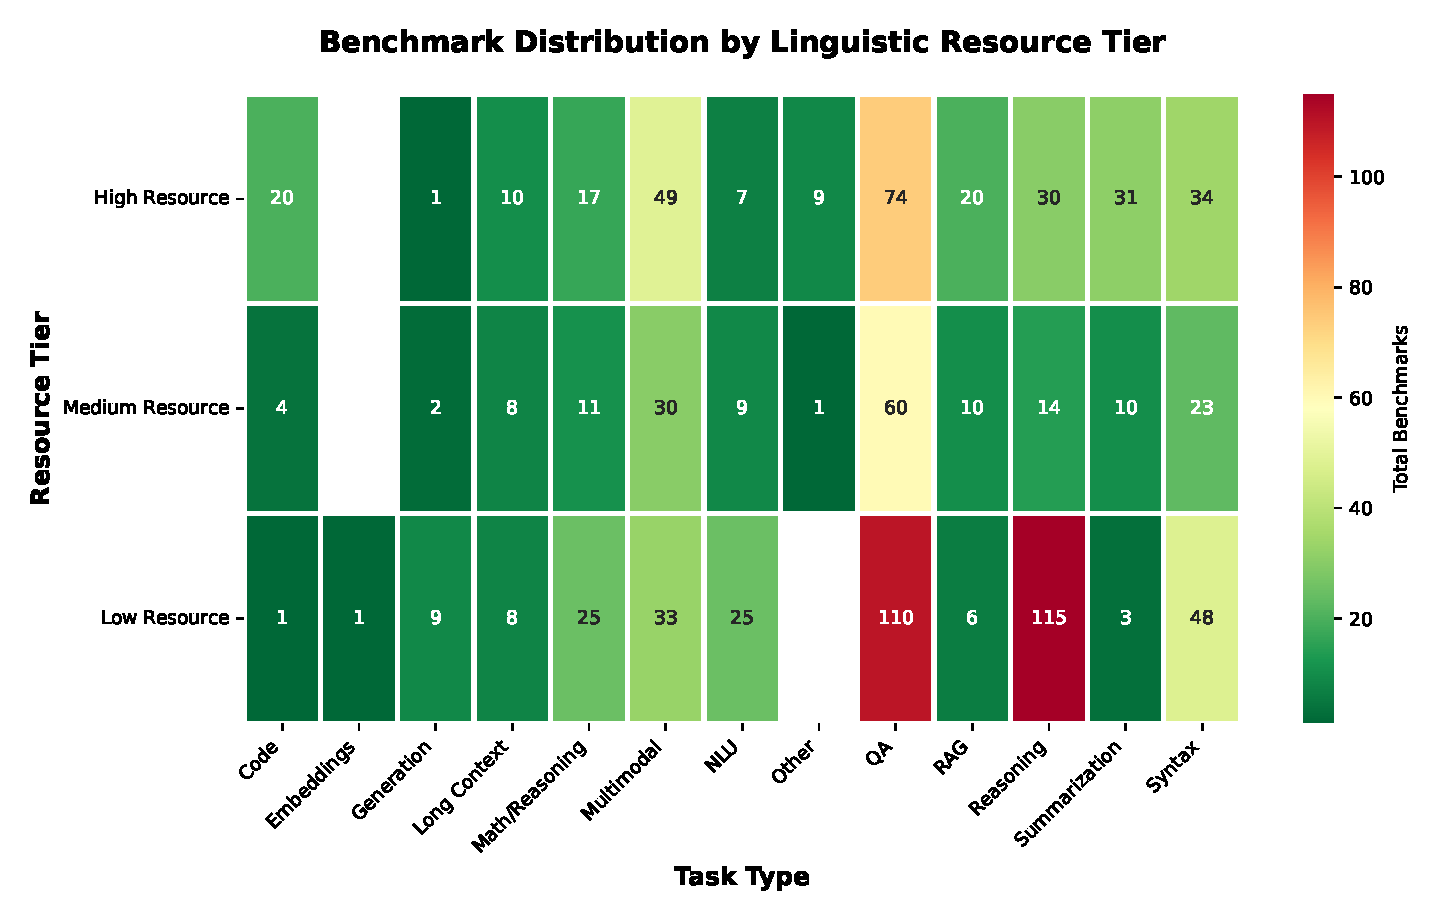
\includegraphics[width=0.8\linewidth]{images/figure3_language_heatmap_tier.pdf}
    \caption{Benchmark coverage by language resource tier. High-resource languages dominate across all task categories, highlighting the need for more low-resource language benchmarks.}
    \label{fig:5_langheatmap}
\end{figure*}


\subsubsection{Math/Reasoning}
\noindent

\citep{shi2022language} investigate whether the chain-of-thought (CoT) reasoning capabilities of large language models (LLMs) extend to languages other than English. While CoT prompting has been shown to elicit strong reasoning performance in English, it was unclear if this ability transfers to other languages, given that LLMs are predominantly trained on English data. To explore this, the authors created the Multilingual Grade School Math (MGSM) benchmark by having native speakers translate 250 problems from the GSM8K dataset into ten typologically diverse languages, including low-resource languages like Bengali and Swahili. The key finding of the work is that LLMs can indeed perform multilingual chain-of-thought reasoning, but this is an emergent property of sufficient model scale. An evaluation of PaLM models showed that the largest model (540B) demonstrated substantial performance gains from CoT prompting across all evaluated languages, even those with minimal representation in the training data, while smaller models did not show a similar benefit. The key strength of this work lies in being the first to demonstrate that the reasoning ability unlocked by CoT prompting is not confined to English, and in providing a new, high-quality benchmark (MGSM) to measure this multilingual capability.

\citep{son2025linguisticgeneralizabilitytesttimescaling} propose MCLM, a multilingual competition-level math benchmark spanning 55 languages, to study whether test-time scaling methods generalize across languages. They evaluate three approaches—Outcome Reward Modeling (ORM), Process Reward Modeling (PRM), and Budget Forcing (BF)—on Qwen2.5-1.5B-Math and a newly trained multilingual reasoning model (MR1-1.5B). Results show that ORM (35.8 on MCLM) and BF with MR1-1.5B (35.2) achieve competitive accuracy, but improvements are largely English-centric (e.g., +20 points on AIME) and average only +1.9 points across other languages. PRM and BF further exhibit unstable performance, amplifying variance and reducing cross-lingual consistency, while “thinking LLMs” constrained to similar inference FLOPs offer no clear advantage over best-of-N selection. The study concludes that, unlike pre-training scaling, test-time scaling does not robustly transfer to multilingual reasoning, and releases MCLM, MR1-1.5B, and evaluation results to support future research

\citep{liu2025maxifemultilingualcrosslingualinstruction} introduce MaxiFE, a framework to improve the efficiency of process supervision in reasoning tasks by reducing annotation cost while retaining performance. Instead of exhaustively labeling reasoning steps, MaxiFE leverages adaptive step selection with two strategies: Length-Based Selection (LBS), which favors shorter solution paths, and Uncertainty-Based Selection (UBS), which prioritizes steps with higher predictive uncertainty. Experiments across GSM8K, MATH, AIME, GPQA, and OlympiadBench using GPT-4.1, Qwen2.5-Math-7B, and LLaMA-3.1-8B show that MaxiFE reduces annotation costs by up to 80\%, while maintaining or even improving accuracy compared to full process supervision. Notably, UBS achieves the best trade-off, yielding comparable performance to fully supervised models with only 20\% of feedback. This work demonstrates that efficient feedback allocation can significantly enhance process supervision, offering a scalable alternative for training reasoning-focused 

\subsubsection{RAG}
\noindent
 \citep{liu2025xragcrosslingualretrievalaugmentedgeneration} introduce XRAG, a benchmark for evaluating LLMs in cross-lingual retrieval-augmented generation (RAG), covering both monolingual retrieval (non-English queries with English-only documents) and multilingual retrieval (queries plus supporting documents in both English and the query language). XRAG is constructed from NewsCrawl (2024) using a multi-step LLM pipeline to generate cross-document Q\&A pairs (aggregation, comparison, multi-hop, set) and includes \textasciitilde 1,500 verified examples across German, Spanish, Chinese, and Arabic. Each instance consists of a question, gold answer, two supporting documents, and six distractors, simulating realistic noisy retrieval. Benchmarking GPT-4o, Claude 3.5, Mistral-Large, Command-R+, and Nova-Pro shows that models achieve only 55–62\% accuracy in monolingual retrieval and $\leq$
58\% in multilingual retrieval, far below human upper bounds (\textasciitilde
85–92\%). Key failure modes include response language correctness errors (answering in English instead of the query language) and difficulty reasoning across multilingual evidence. XRAG highlights that even frontier models struggle with cross-lingual RAG, providing the first benchmark to systematically study this setting.

\subsubsection{Code}
\noindent

\citep{raihan-etal-2025-mhumaneval} present mHumanEval, a massively multilingual benchmark for code generation that extends HumanEval from 164 English-Python tasks to 33,456 prompts across 204 natural languages (NLs) and 25 programming languages (PLs), including four new PLs (MATLAB, Visual Basic, Fortran, COBOL). Prompts were translated using GPT-4o, NLLB, and Google Translate, with quality filtered via BERTScore and CometKiwi, and supplemented with expert human translations in 15 languages. The benchmark provides multiple subsets (e.g., mHumanEval-mini, T500, B500) and supports broad evaluations. Experiments with six SOTA models (GPT-4o, Claude-3.5, GPT-3.5, DeepSeek-Coder, WizardCoder, Aya) reveal that closed-source models (GPT-4o, Claude-3.5) achieve the most consistent Pass@1 performance across high- and low-resource languages, while specialized code models like WizardCoder excel in English but collapse in low-resource and non-Python settings. Error analysis highlights failures due to mistranslation (e.g., Zulu “prime number” → “significant number”) and keyword leakage into target NLs. The study concludes that multilingual pretraining is critical for cross-lingual code generation, and releases the full benchmark to enable scalable evaluation.


\cite{sato-etal-2024-cl} introduce CL-HumanEval, a benchmark for evaluating cross-lingual transfer in code generation, extending HumanEval and JHumanEval while explicitly removing confounding hints (function names, variable names, execution examples) to isolate the role of natural language descriptions. To ensure multilingual fairness, docstrings were rewritten with LLMs and translated into Japanese with human quality control, producing a dataset consistent across languages. Experiments on Gemma, CodeGemma, LLaMA-2, CodeLLaMA, and LLaMA-3 show that CL-HumanEval yields lower but more accurate scores than HumanEval/JHumanEval, since models cannot rely on structural hints; English performance generally exceeds Japanese, reflecting training-data imbalance, but results confirm CL-HumanEval’s sensitivity to cross-lingual differences. Additional experiments with Japanese continual pre-training and instruction tuning reveal limited improvements and in many cases catastrophic forgetting, further validating the benchmark’s utility for probing how training strategies impact cross-lingual transfer.

\subsubsection{Generation}
\noindent

\citep{} introduces a unified framework for multilingual evaluation of large language models (LLMs)
11-CIA Suite. It consists of (i) HERCULE, a family of cross-lingual, reference-based evaluator LLMs, and (ii) RECON, a human-annotated benchmark spanning six languages (Bengali, German, French, Hindi, Telugu, Urdu) with 500 diverse prompts covering reasoning, planning, creativity, safety, and instruction-following tasks. Unlike existing metrics that are English-centric, HERCULE leverages English reference answers to evaluate model responses in other languages, addressing the scarcity of non-English references. Trained on the INTEL dataset (100k translated examples), HERCULE shows stronger alignment with human judgments than proprietary models like GPT-4O and Gemini-1.5-Pro, particularly in low-resource settings. Extensive ablations demonstrate its effectiveness in zero-shot cross-lingual transfer, the importance of reference answers, and the utility of LoRA and weight-merging techniques for resource efficiency. By making code, models, and datasets publicly available, CIA Suite provides a scalable and reproducible approach for benchmarking and meta-evaluating multilingual LLMs


\citep{singh2024indicgenbenchmultilingualbenchmarkevaluate} benchmark is the largest multilingual generation evaluation suite for Indic languages, spanning 29 languages, 13 scripts, and 4 language families. It covers five key user-facing generation tasks: cross-lingual summarization (CROSSSUM-IN), machine translation (FLORES-IN), multilingual QA (XQUAD-IN), and cross-lingual QA (XORQA-IN-XX/EN). Unlike prior Indic resources, it provides multi-way parallel, professionally translated evaluation datasets, with first-time coverage for up to 18 low-resource languages such as Manipuri, Santali, and Bodo. Evaluation of open-source (mT5, LLaMA, BLOOMZ, Gemma) and proprietary models (GPT-3.5, GPT-4, PaLM-2) reveals consistent performance gaps between English and Indic languages, with PaLM-2-L achieving the strongest results but still underperforming significantly in low-resource settings. Additional analyses highlight challenges from tokenization disparities, high fertility in mid/low-resource languages, hallucinations, and language mixing, underscoring the need for fairer tokenization schemes and culturally grounded modeling. By releasing both evaluation and limited training data, IndicGenBench enables fine-tuning, in-context learning, and cross-lingual transfer experiments, establishing itself as a comprehensive benchmark for generative LLMs in Indic languages

\subsubsection{Long Context}
\citep{kim2025rulermeasureallbenchmarking} extend the English-only RULER framework into a multilingual long-context evaluation suite covering 26 languages. It introduces seven synthetic tasks—five variants of the needle-in-a-haystack (NIAH) retrieval challenge, including a novel nonexistent needle setting, and two aggregation tasks (Common Word Extraction, easy/hard)—to test both retrieval and reasoning abilities across context lengths up to 128K tokens. Instructions were written in English and translated by native speakers into 25 other languages, spanning diverse families and scripts. Evaluation of open-weight (Qwen2.5, LLaMA 3.1/3.3, DeepSeek-R1) and closed-source models (Gemini-1.5 Flash, OpenAI o3-mini-high) reveals several surprising findings: (i) performance gaps between high- and low-resource languages widen as context length increases, (ii) English is not top-performing, ranking 6th overall at long contexts, with Polish outperforming all others, (iii) models frequently fail when tasked with recognizing the absence of a needle, and (iv) aggregation tasks remain unsolved, with <1\% accuracy on the hardest variant. Cross-lingual evaluations further show that the instruction language can shift accuracy by up to 20\%, underscoring the interplay between instruction tuning and language coverage. ONERULER thus provides a rigorous, multilingual, and cross-lingual diagnostic benchmark for probing long-context reasoning in LLMs, highlighting both current limitations and directions for multilingual training

\subsubsection{Embedding}
\noindent

 \citep{enevoldsen2025mmtebmassivemultilingualtext} propose the largest evaluation suite for multilingual text embeddings, extending MTEB to over 500 tasks across 250+ languages. It covers ten task categories—including retrieval, clustering, bitext mining, classification, semantic textual similarity, and instruction following—spanning diverse domains such as fiction, medical, social media, and programming. To ensure inclusivity, MMTEB was built through a large-scale open collaboration with native speakers and researchers, implementing systematic quality checks. A key contribution is benchmark optimization for accessibility: by downsampling tasks (e.g., TREC pooling for retrieval, bootstrapping for clustering) and caching embeddings, MMTEB reduces compute costs by up to 100× while preserving model ranking fidelity (Spearman $\geq$ 0.9). The benchmark includes specialized subsets—MTEB(Multilingual), MTEB(Europe), MTEB(Indic), and MTEB(eng v2)—allowing regional and domain-specific evaluation. Results show that while 7B LLM-based embedding models (e.g., GritLM-7B, e5-Mistral-7B-Instruct) achieve state-of-the-art retrieval, smaller XLM-R-based models (multilingual-e5-large-instruct, 560M) outperform them on low-resource languages, highlighting the trade-off between scale and multilingual generalization. By releasing code, datasets, and a public leaderboard, MMTEB establishes a scalable, community-driven standard for multilingual embedding evaluation

\subsubsection{Others}
\noindent

\citep{adelani2024irokobench} present IrokoBench, a comprehensive benchmark designed to evaluate the capabilities of Large Language Models (LLMs) on culturally and linguistically relevant tasks for African languages. The advancement of LLMs for the African continent is hindered by the scarcity of high-quality evaluation benchmarks, with most existing multilingual datasets offering poor coverage or relying on culturally biased, translated English content. To address this, the authors curated a benchmark consisting of 15 diverse natural language understanding and generation tasks, including question answering, summarization, and named entity recognition, across 20 major African languages. The key feature of IrokoBench is that it is constructed entirely from natively created datasets developed by African researchers and native speakers, ensuring that the tasks are authentic and reflect the specific linguistic and cultural contexts of the continent. A comprehensive evaluation of over 30 LLMs, including proprietary models like GPT-4o and African-centric models, reveals that while proprietary models generally lead, all models exhibit a significant performance gap compared to their capabilities in English, and performance varies widely across different African languages and tasks. The key strength of this work lies in providing the first large-scale, culturally-grounded benchmark suite for African languages built from native data, which establishes a more authentic and reliable standard for measuring progress and guiding the development of more equitable AI technology for Africa.


\citep{asai2023buffetbenchmarkinglargelanguage} propose BuffettPrompt, a framework to enhance multi-turn reasoning in LLMs by treating prompts as an “all-you-can-eat buffet” where models dynamically allocate tokens across reasoning steps. Instead of fixed-length reasoning or static prompting, BuffettPrompt introduces a token allocation mechanism that adaptively expands or contracts reasoning based on task complexity. The method is benchmarked on GSM8K, MATH, AIME, GPQA, and OlympiadBench with models including GPT-4.1, Qwen2.5-Math-7B, and LLaMA-3.1-8B, showing that BuffettPrompt outperforms chain-of-thought and best-of-N baselines, achieving stronger accuracy with significantly fewer tokens on average. Results demonstrate that efficient dynamic prompting can reduce compute cost while improving reasoning robustness, making BuffettPrompt a practical alternative for scaling test-time reasoning.

















\section{Discussion}

Our systematic analysis of 65 evaluation benchmarks and 31 training datasets reveals a multilingual AI landscape that is rapidly expanding yet marked by significant imbalances. While the recent surge in resource creation, particularly in 2024-2025, signals a positive trend, our five-dimensional taxonomy uncovers critical gaps that challenge the pursuit of globally reliable and equitable AI. This section discusses the implications of these findings, highlighting disparities in linguistic coverage, task representation, and cultural grounding.

\subsection{The Pervasive Skew Towards High-Resource Languages}

A primary finding of our study is the profound concentration of evaluation resources on a handful of high-resource languages. As illustrated in our language coverage analysis, languages like English, Chinese, Spanish, and French dominate the landscape, while a long tail of low-resource languages remains severely underrepresented. Over 70\% of both benchmarks and datasets are classified as high-resource (Table 1). This disparity creates a significant risk of developing models that perform well on a few dominant languages but fail catastrophically on the vast majority of the world's linguistic diversity \citep{blodgett-etal-2020-language}. The reliance on machine-translated content for many benchmarks (26.2\%) further exacerbates this issue, as translation artifacts can mask true model capabilities and introduce biases \citep{smith2024implementingonlinereinforcementlearning}. Our findings serve as a quantitative call to action for the community to prioritize the creation of native, high-quality benchmarks for low-resource languages, moving beyond the current Anglocentric paradigm.

\subsection{Imbalances in Task and Capability Evaluation}

Our taxonomy reveals a thematic imbalance in the capabilities being evaluated. Question Answering (QA) and Syntactic tasks together account for nearly 50\% of all evaluation benchmarks. While important, this focus leaves other critical capabilities undertested. Complex reasoning, cultural understanding, safety, and multimodal grounding are represented by only a handful of benchmarks. This narrow evaluative focus may lead to an incomplete understanding of model performance and could encourage the development of models with brittle, task-specific knowledge rather than robust, generalizable intelligence. The community must diversify its evaluation portfolio to encompass a broader range of cognitive and social capabilities to ensure models are not only accurate but also safe, robust, and contextually aware.

\subsection{The Neglected Dimension of Cultural Grounding}

Perhaps the most significant gap identified is the lack of cultural grounding in existing benchmarks. A majority of resources (55.4\% of benchmarks, 71.0\% of datasets) are designed to be "Universal," stripping away the cultural context that is intrinsic to human language. While this approach has its merits for certain tasks, it neglects the fact that language is a deeply cultural construct. Models trained and evaluated on culturally-agnostic data are likely to fail in real-world applications where cultural norms, values, and contexts are paramount \citep{10.1162/tacl_a_00760}. The small number of "Culturally Anchored" (26.2\%) and "Region-Specific" (18.5\%) benchmarks is a critical deficiency. We argue that future work must move beyond simple linguistic translation and embrace the creation of benchmarks that are deeply embedded in diverse cultural contexts, which is essential for developing truly globally competent AI systems.

\subsection{Limitations}

We acknowledge several limitations in our work. First, while we conducted an extensive search, our corpus of 96 resources is not exhaustive and represents a snapshot of a rapidly evolving field. Second, the categorization along our five dimensions, particularly for cultural grounding and task type, involves a degree of subjective interpretation. We have made our complete dataset and classification criteria publicly available to ensure transparency and encourage community refinement. Finally, our analysis focuses on the existence of benchmarks, not their widespread adoption or quality, which are important areas for future research.



\section{Conclusion}

In this work, we introduced a systematic, five-dimensional taxonomy for multilingual AI evaluation and applied it to a comprehensive corpus of 65 evaluation benchmarks and 31 training datasets. Our analysis provides a detailed map of the current landscape, revealing not only its rapid growth but also its critical imbalances. We identified significant skews towards high-resource languages, a narrow focus on a few task types, and a widespread neglect of cultural context.

These findings underscore an urgent need for the AI community to move beyond English-centric and culturally-agnostic evaluation paradigms. To build AI that is truly reliable, equitable, and beneficial for a global population, we must consciously and deliberately invest in creating diverse, culturally-grounded, and linguistically-representative benchmarks. This work provides a foundational framework and a quantitative baseline to guide and measure that effort. We release our complete dataset and analysis publicly, inviting the community to build upon this taxonomy and join in the collective endeavor to foster a more inclusive and robust future for multilingual AI.

\section*{Acknowledgments}

We are grateful to the multilingual NLP research community for their continued efforts in creating and maintaining the benchmarks and datasets analyzed in this work. We particularly thank the creators of the resources included in our taxonomy for making their work publicly available and advancing the field of multilingual AI evaluation.


%%
%% The next two lines define the bibliography style to be used, and
%% the bibliography file.
\bibliographystyle{ACM-Reference-Format}
\bibliography{custom}


%%
%% If your work has an appendix, this is the place to put it.
\appendix

\end{document}
\endinput
%%
%% End of file `sample-acmsmall.tex'.
